\title{Lattice quantum chromodynamics}\label{chap:latticeqcd}
\author{Tetsuo Hatsuda} 
\institute{Tetsuo Hatsuda \at Nishina Center, RIKEN, Saitama 351-0198, Japan,  \email{thatsuda@riken.jp}}
\maketitle
\abstract{
%Each chapter should be preceded by an abstract (10--15 lines long) that summarizes the content. The abstract will appear \textit{online} at \url{www.SpringerLink.com} and be available with unrestricted access. This allows unregistered users to read the abstract as a teaser for the complete chapter. As a general rule the abstracts will not appear in the printed version of your book unless it is the style of your particular book or that of the series to which your book belongs.\newline\indent
%Please use the 'starred' version of the new Springer \texttt{abstract} command for typesetting the text of the online abstracts (cf. source file of this chapter template \texttt{abstract}) and include them with the source files of your manuscript. Use the plain \texttt{abstract} command if the abstract is also to appear in the printed version of the book.
Concepts and applications of lattice quantum chromodynamics (LQCD) are introduced.
After discussing how to define quarks and gluons on the Euclidean hypercubic lattice, 
 the strong coupling expansion  and the weak coupling expansions are reviewed 
 to see the vital role played by the quantum fluctuations in QCD.
 Fundamental techniques for numerical LQCD simulations  such as the Markov Chain Monte Carlo method and the
  Hybrid Monte Carlo method are discussed in some details.  As 
  examples of the high precision LQCD simulations,  numerical results of the heavy quark potential and the hadron masses
   are shown.  Recent LQCD results on the baryon-baryon interactions are briefly discussed.
   }

% macros %%%%%%%%%%%%%%%%%%%%%%%%%%%%%%%%%%%
%\renewcommand{\theequation}{\thesection.\arabic{equation}}
\newcommand{\beq}{\begin{eqnarray}}
\newcommand{\eeq}{\end{eqnarray}}
\newcommand{\la}{\langle}
\newcommand{\ra}{\rangle}
%% vector-notation
\newcommand{\vx}{\vec{x}}
\newcommand{\vy}{\vec{y}}
\newcommand{\vk}{\vec{k}}
\newcommand{\LRDelta}{\overleftrightarrow{\Delta}}
\newcommand{\vgamma}{\vec{\gamma}} 
\newcommand{\vA}{\vec{A}}
\newcommand{\vr}{\vec{r}}
\newcommand{\vn}{\vec{n}}
\newcommand{\vm}{\vec{m}}
\newcommand{\vv}{\vec{v}}
\newcommand{\vp}{\vec{p}}
\newcommand{\vsigma}{\vec{\sigma}}
\newcommand{\vL}{\vec{L}}
\newcommand{\vS}{\vec{S}}
\newcommand{\vT}{\vec{T}}
%% lattice
\newcommand{\Rs}{R_{\rm s}}
\newcommand{\Rt}{R_{\rm t}}
\newcommand{\Ns}{N_{\rm s}}
\newcommand{\Ntau}{N_{\tau}}
\newcommand{\at}{a_{\rm t}}
\newcommand{\as}{a_{\rm s}}
\newcommand{\Lamqcd}{ \Lambda_{_{\rm QCD}} } 
\newcommand{\Lamlat}{ \Lambda_{_{\rm LAT}} } 
\newcommand{\Lammsb}{ \Lambda_{_{\overline{\rm MS} }}  } 
%%%%%%%%%%%%%%%%%%%%%%%%%%%%%%%%%%%%%%%%%%%%%



%%%%%%%%%%%%%
\section{Introduction}
%%%%%%%%%%%%%

In this chapter, we introduce  lattice quantum chromodynamics (LQCD) 
originally proposed by K. Wilson in 1974 \cite{Wilson:1974sk}. What makes the LQCD unique and powerful is that
it can allow first-principle,  gauge invariant and non-perturbative calculations of strongly interacting
quarks and gluons.  After the first numerical attempts by M. Creutz \cite{Creutz:1980zw},
 LQCD simulations have been extensively applied to study heavy quark potentials,
hadron masses,  hadronic matrix elements, QCD phase transition at finite temperature, 
and so on.  In recent years, there are also progresses 
in deriving the  baryon-baryon interactions, which are particularly relevant to 
nuclear physics and astrophysics. Throughout this chapter, we will focus on the theoretical concepts, numerical techniques and some
applications to hadron masses and nuclear forces.  LQCD at finite temperature and/or baryon density will
not be covered.  The interested readers may want to consult the  following review articles for further details, or may even 
want to run the open source codes or to use the open LQCD configurations.

\vspace{0.3cm}

 \noindent
 {\bf Review articles:}   Here is a list a few articles which are useful to learn more about LQCD.  
 \begin{itemize}
\item Comprehensive review on QCD can be seen in \cite{Brambilla:2014jmp}.
\item The origin of LQCD is discussed in \cite{Wilson:2004de}.
\item The basic concepts  of LQCD are summarized in the monographs \cite{Creutz:1984mg,Rothe:1992nt}.
 \item Recent progresses of LQCD can be seen in the reviews \cite{Hoelbling:2014uea,Ukawa:2015eka} and references therein. 
 \end{itemize}

\vspace{0.3cm}

 \noindent
 {\bf Open source codes:} 
 It takes a lot of time and energy to develop the LQCD code from scratch. To lower the bar,
 several source codes for LQCD simulations have been released for public use.
  \begin{itemize}
\item Bridge++: \url{http://bridge.kek.jp/Lattice-code/index_e.html}
\item Lattice ToolKit: \url{http://nio-mon.riise.hiroshima-u.ac.jp/LTK/}
\item OpenQCD: \url{http://luscher.web.cern.ch/luscher/openQCD/index.html}
\item USQCD: \url{http://usqcd-software.github.io/}
\end{itemize}

\vspace{0.3cm}
 \noindent
{\bf LQCD configurations:}  Outputs of large scale LQCD simulations  is a {\it big data}  
called "LQCD configurations".   Physicists can study various aspects of QCD by using these configurations.
 The International Lattice Data Grid (ILDG) is a project to share the configurations around the world.
  \begin{itemize}
 \item ILDG \url{http://plone.jldg.org/wiki/index.php/Main_Page}
\end{itemize}
 
%================================
  \subsection{Euclidean QCD action}
%================================
LQCD is formulated on the Euclidean spacetime lattice.
Observables in the Minkowski spacetime are obtained by the analytic continuation of the 
imaginary-time $\tau$ to the real-time $t$.  In terms of the time evolution operator in quantum mechanics,
it corresponds to the continuation from the imaginary time evolution, $e^{-H \tau} $, to the real time
evolution, $e^{-iHt}$, where $H$ being the Hamiltonian of the system.  The functional integral representation of the 
the Euclidean QCD partition function ${\cal Z}$  on a finite spatial box $L^3$  and the temperature $T$ is given by
\beq
\label{eq:Z-QCD}
{\cal Z}(T,V,J) = \int [dA d\bar{q} dq] e^{- \int_{0}^{1/T}  d\tau \int_{L^3} d^3 x \left( {\cal L}_{\rm QCD}^{\rm E} + J \Xi \right) }
\eeq
where the Euclidean QCD Lagrangian in terms of quarks $q^{\alpha=1,2,3}$ and gluons $A_{\mu=1,2,3,4}^{b=1, \cdots, 8}$ 
is given by
\beq
{\cal L}_{\rm QCD}^{\rm E} = \bar{q}^{\alpha} (\Gamma_{\mu}  D_{\mu}^{\alpha \beta} + m \delta^{\alpha \beta}) q^{\beta} 
+ \frac{1}{4} G_{\mu \nu}^b G_{\mu \nu}^b,
\eeq
Here the Euclidean version of the $\gamma$-matrices, $\Gamma_\mu$, is defined in
 the Appendix [Four vectors and Dirac matrices].
The quark mass matrix in the flavor space ($u, d, s, \cdots$) is denoted by $m$ with the flavor indices suppressed.
 The color covariant derivative is defined by
\beq
D_{\mu}^{\alpha \beta} = \partial_{\mu} \delta^{\alpha \beta} + ig A_{\mu}^{\alpha \beta}, 
\eeq
with  $x_{\mu}= (\tau, \vx)$,  $\partial_{\mu} = (\partial_{\tau}, \nabla )$ and the $3 \times 3$ matrix field, $A_{\mu} = A_{\mu}^b t^b$. 
The explicit form of the color SU(3) generators $t^{a=1, \cdots, 8}$ is given in the Appendix [SU$(N)$ algebra]. 
The field strength tensor is $G_{\mu \nu}=G_{\mu \nu}^b t^b$ with
 $G_{\mu \nu}^b= \partial_{\mu}A_{\nu}^b - \partial_{\nu} A_{\mu}^b -g f_{bcd} A_{\mu}^c A_{\nu}^d$.
 The arbitrary external fields (such as the external source of the quarks and gluons,
 external electroweak fields etc) are denoted by $J$, while the corresponding dynamical operators 
  are denoted by $\Xi (A, \bar{q}, q)$.  The functional integration measure for the 
 c-number gluons and the Grassmann-number quarks is defined by
 \beq
 [dA d\bar{q} dq] \equiv \prod_{x, {\rm color, spin, flavor}}  dA_{\mu}^b(x) d\bar{q}^{\alpha}(x)  dq^{\beta} (x).
\eeq 
See Appendix [Gaussian and Grassmann integrals] for the examples of integration with these measures.
The temporal boundary condition of the gluon (quark) field is periodic (anti-periodic) due to its
c-number (Grassmann-number) character;  $A_{\mu}^b (\tau=0, \vx)=A_{\mu}^b (\tau=1/T, \vx)$,
$\bar{q}^{\alpha}(\tau=0,\vx)=-\bar{q}^{\alpha}(\tau=1/T,\vx)$, and 
$q^{\beta}(\tau=0,\vx)=-q^{\beta}(\tau=1/T,\vx)$.    On the other hand, the spatial boundary conditions are 
not constrained and can be taken to be either periodic or anti-periodic; the difference should disappear in the 
thermodynamic limit, $L \rightarrow \infty$.
 Throughout this chapter, we take $T = 1/L $   to
  study hadrons and hadron-hadron interactions at zero temperature in the thermodynamic limit.

Further details of the functional integral formulation of the general many-body systems of fermions and bosons
can be seen in the textbook \cite{Negele:1988vy}.

%================================
 \subsection{Quantum fluctuations}
%================================
In weak coupling perturbation theory, one assumes that the QCD coupling $g$  is small and expand the partition function
 ${\cal Z}$ in terms of a power series of $g$.  Such a perturbative expansion in QCD is justified, however, only in  limited 
 circumstances  such as at extreme high  temperature/density  or at very short distances. This is because  the 
  renormalized QCD coupling (or often called the running coupling) becomes small only in the processes 
  with the energy scale much above 1 GeV. This is called the asymptotic freedom.
 To calculate low-energy hadron properties below 1 GeV,
  we need to go beyond perturbation theory and to evaluate the functional integral with full quantum fluctuations.
 The lattice QCD provides a way to carry out this task numerically in a gauge invariant manner. 
 

  
%%%%%%%%%%%%%%%%%%%%%%
\section{Lattice QCD: theoretical basis } 
%%%%%%%%%%%%%%%%%%%%%%

%================================
\subsection{Wilson line}
%================================

% FIG %%%%%%%%%%%%%%%%%%%%%%%%%%
\begin{figure}[t]
\begin{center}
%\framebox[74mm]{\rule[-26mm]{0mm}{52mm}}
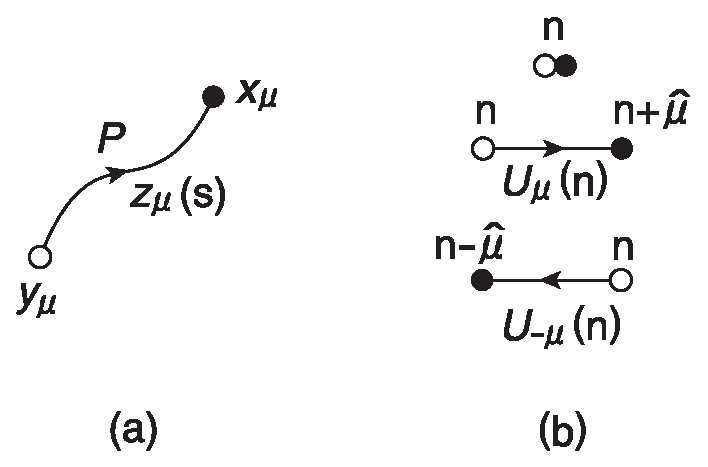
\includegraphics[scale=0.6]{Chapter3-figures/wilson-line.eps}
 \end{center}
\caption{(a) The Wilson line in the Euclidean spacetime. (b)
 Basic quark bilinears with gauge invariance.}
\label{fig:wilson-line}
\end{figure}
%%%%%%%%%%%%%%%%%%%%%%%%%%%%%


Let us first start with the {\it Wilson line} which is defined on 
  a path $P$ connecting the point $y$  and $x$ in the continuous Euclidean spacetime 
   as shown in Fig.\ref{fig:wilson-line}(a).
By parametrizing the path in terms of a coordinate
   $z(s)$ with $z(s=0)= y$ and $z(s=1)=x$, the Wilson line reads
\beq
\label{eq:5.wilson-line}
U_P(x,y;A) & = & 
{\rm P} \ {\rm exp} \left( ig \int_P dz_{\mu} A_{\mu} \right)
={\rm P} \ {\rm exp} \left( ig \int_0^1 ds\ \lambda_{\mu}
 A_{\mu} \right)
  \nonumber \\
  &  & \! \! \! \! \!  
  \! \! \! \! \! \! \! \! \! \! \! \! \! \! = \sum_{n=0}^{\infty} 
 {(ig)^n \over n!} \int_0^1 ds_1 \int_0^1 ds_2 \cdot \cdot \cdot \int_0^1 ds_n \ 
 {\rm P}[\lambda \cdot A(s_1)\ \cdot \cdot \cdot \
  \lambda \cdot A(s_n)],
 \eeq
 where   
 $\lambda_{\mu} = dz_{\mu}/ds$. The path ordered symbol ${\rm P}$ is 
  necessary because $A_{\mu} = A_{\mu}^a t^a$ is a 
  matrix in the color space.   
 
  The Wilson line has the following  properties
   which can be proved from  the definition of $U_P$ (Exercise \ref{prob:1}) :
\begin{enumerate}
  \item[(i)]  It can be broken into parts at any arbitrary points on the path;
\beq
\label{eq:5.wilson-line-i}
U_P(x,y;A) = U_{P_2}(x,z(s);A) U_{P_1}(z(s),y;A).
\eeq
\item[(ii)] It satisfies a differential equation,
\beq
\label{eq:5.wilson-line-ii}
{d \over ds} U_P(z(s),y;A)= 
 \left[ ig \lambda(s)\cdot  A(z(s)) \right] \ U_P(z(s),y;A).
\eeq
\item[(iii)] Under the local gauge transformation  
$A_{\mu}^V(x) = V(x)[A_{\mu}(x) V^{\dagger}(x) -(i/g) V(x) (\partial_{\mu}  V^{\dagger}(x))$, 
 it transforms covariantly, 
\beq
\label{eq:5.wilson-line-iii}
U_P(x,y;A) \rightarrow U_P(x,y;A^V) = V(x) U_P(x,y;A) V^{\dagger}(y).
\eeq
 \end{enumerate}

The Wilson line is useful to define the non-local and gauge-invariant objects.
In particular, the gauge-invariant quark bilinear
$\bar{q}(x) U_P(x,y;A) q(y)$, and the gauge-invariant {\it Wilson loop}
 ${\rm tr} \ U_P(x,x;A)$ turn out to be important building blocks to define
   the QCD action on the lattice.  Here ``tr" implies the trace 
 over  color indices.
   
%===========================  
\subsection{Lattice gluons}  
%===========================

% FIG %%%%%%%%%%%%%%%%%%%%%%%%%%
\begin{figure}[t]
\begin{center}
%\framebox[74mm]{\rule[-26mm]{0mm}{52mm}}
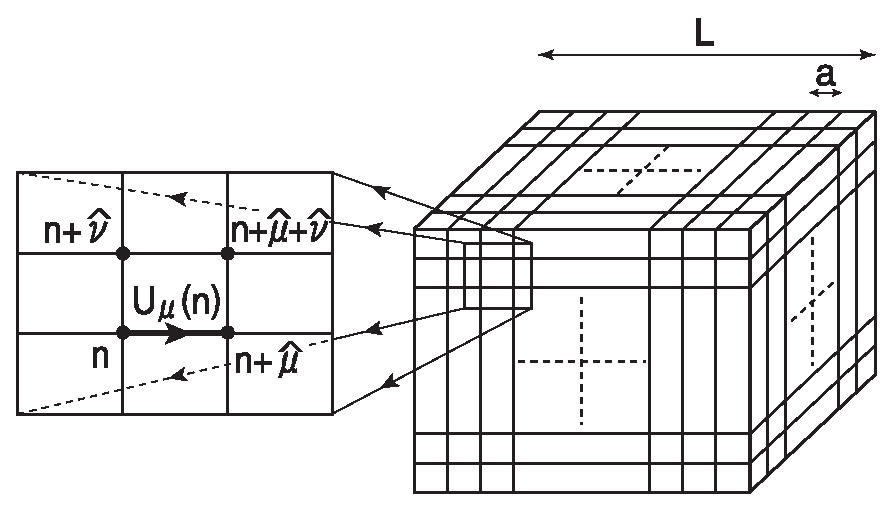
\includegraphics[scale=0.6]{Chapter3-figures/cube.eps}
 \end{center}
\caption{A hypercubic lattice in Euclidean spacetime with
 a lattice constant $a$ and the lattice size $L$.
 Quarks $q(n)$ (gluons $U_{\mu} (n)$ ) are
 defined on the sites (links).}
\label{fig:cube}
\end{figure}
%%%%%%%%%%%%%%%%%%%%%%%%%%%%%%


Let us consider a four dimensional  hyper-cubic lattice
 with a lattice spacing $a$ and the four dimensional volume $L^4$.
 Each lattice site is specified by  $n_{\mu}$ corresponding to the
 Euclidean coordinates through $x_{\mu} = a n_{\mu}$ (see Fig.\ref{fig:cube}).
   The {\it link variable} (the shortest  Wilson line on the lattice) is an SU(3)
 matrix connecting the neighboring sites $n$ and $n + \hat{\mu}$,
\beq
\label{eq:5.wilson-link}
U_{\mu}(n) = {\rm exp} \left(  ig a A_{\mu} (n) \right) .
\eeq
 Here $\hat{\mu}$ implies a vector  pointing the 
 direction of $\mu$ with a length $a$. 
 Since it is the minimal
     Wilson line, we do not need the path ordering symbol ${\rm P}$.
   Also, any non-minimal Wilson line on the lattice  is represented by a
    product of link-variables.  For later purpose, we introduce the link variable pointing the 
    opposite direction as  $U_{-\mu}(n+\hat{\mu}) = [U_{\mu}(n)]^{\dagger}$.

Let us now  define the smallest closed loop;
\beq\label{eq:5.wilson-plaq}
 U_{\mu \nu}(n) = 
 U_{\nu}^{\dagger}(n) U_{\mu}^{\dagger}(n+ \hat{\nu} ) 
  U_{\nu}(n+ \hat{\mu} )U_{\mu}(n ).
\eeq
Under local gauge
 transformation (rotation under  arbitrary  SU(3) matrix $V(n)$), we have 
\beq
 U_{\mu}(n) \rightarrow  V(n) U_{\mu}(n) V^{\dagger}(n+\hat{\mu}), \ \ 
 U_{\mu \nu}(n) \rightarrow  U_{\mu \nu}^V(n)=V(n) U_{\mu \nu}(n) V^{\dagger}(n),
 \eeq
which are the  direct consequence of Eq.(\ref{eq:5.wilson-line-iii}).

In the naive continuum limit where $a \rightarrow 0$, we have
\beq
 \label{eq:5.wilson-plaq-cont}
 U_{\mu}(n) -1 
   &=& iga A_{\mu}(n)  + O(a^2), \\
 \label{eq:5.wilson-plaq-cont-2}
 U_{\mu \nu}(n) -1 
  &=& \exp \left( iga^2 t^b (G_{\mu \nu}^b(n) + O(a^3) ) \right) -1
  = ig a^2 G_{\mu \nu}(n)  + O(a^4), \\
{\rm tr} \left(    U_{\mu \nu}(n) -1 \right) 
 &=&   {\rm tr} \left[  iga^2 t^b (G_{\mu \nu}^b(n) + O(a^3)) - \frac{1}{2} g^2 a^4 G_{\mu \nu}(n)^2 + O(a^5) \right] \nonumber \\ 
 &=& - \frac{1}{4} g^2 a^4 (G_{\mu \nu}^b(n))^2 + O(a^5) .
\eeq
Here  Eq.(\ref{eq:5.wilson-plaq-cont-2}) is obtained by 
 using the Baker-Campbell-Hausdorff formula, 
  ${\rm exp}X\cdot {\rm exp}Y =
  {\rm exp}(X + Y + [X,Y]/2 + \cdot \cdot \cdot )$.  (Exercise \ref{prob:2}). 


Finally, 
a  gluon action on the lattice, which reduces to the Yang-Mills
 action in the leading order of the  naive continuum limit ($a \rightarrow 0$), reads
\beq
\label{eq:5.wilson-action-cont}
 S_{\rm G}  &=& \beta \sum_{\rm Pl} \left[ 1 - \frac{1}{N_c} {\rm Re} \ {\rm tr} \ U_{\mu \nu}(n) \right] \\
 &=& \beta  a^4 \sum_n \sum_{\mu < \nu} \left[ 1 - \frac{1}{2N_c} {\rm tr}  \left( U_{\mu \nu}(n) +  U_{\mu \nu}^{\dagger}(n) \right) \right] \nonumber \\
 & = & \frac{1}{g^2} \sum_n \sum_{\mu \neq \nu} {\rm tr} \left[ 1 -U_{\mu \nu} (n) \right] 
  \ \ \ \ \xrightarrow{a\rightarrow 0}   \ {1 \over 4} \int d^4x  \ G_{\mu \nu}^b (x)^2 , \nonumber
 \eeq
where $\sum_{\rm Pl} $ is a sum over all non-oriented {\it plaquettes} (minimum square tile on the lattice with the area $a^2$). 
Note that  $\beta \equiv \frac{2N_c}{g^2}$ with $N_c$ being the number of colors ($N_c=3$ for QCD) 
 should not be  confused with the inverse temperature. 
    The lattice gluon action is not unique in the sense
 that one may add arbitrary non-minimal terms which vanish
 in the continuum limit ($a\rightarrow 0$).
  
%============================
\subsection{Lattice fermions}
%============================

There exist three types of gauge invariant objects made of nearest neighbor fermions as shown in Fig.\ref{fig:wilson-line}(b);
\beq
\label{eq:5.nn-link}
\bar{q}(n) q(n), \ \ 
\bar{q}(n+\hat{\mu}) U_{\mu}(n) q(n), \ \
\bar{q}(n-\hat{\mu}) U_{-\mu}(n) q(n).
\eeq
Here one may put any $\gamma$-matrices  between $\bar{q}$ and $q$
 without spoiling the color gauge invariance.
A special combination of the above   terms is called the Wilson's fermion action 
\beq
\label{eq:5.wilson-fermion}
\! \! \! 
S_{\rm F}
 &=& a^4 \sum_n 
  \left[
    m   \bar{q}(n)q(n) - \frac{1}{2a}
    \sum_{\pm \mu} \bar{q}(n+\hat{\mu}) {\Gamma}_{\mu} U_{\mu}(n) q(n)   
    - \frac{r}{2a} \sum_{\pm \mu}   \left( \bar{q}(n+\hat{\mu}) U_{\mu}(n) q(n) - \bar{q}(n)q(n) \right) 
  \right]  \nonumber \\ 
\label{eq:5.wilson-fermion2}
 & \equiv & a^4 \sum_{n',n} \bar{q}(n')
 \left( m \delta_{n',n} + D_{_{\rm W}}(n',n;U) \right) q(n)  \\
 \label{eq:5.wilson-fermion3}
 & & \xrightarrow[a \rightarrow 0] \ \  \int d^4x\  \bar{q} (x)  \left(\Gamma_{\mu} D_{\mu} + m - \frac{ar}{2} D_{\mu}^2 \right)   q(x),
\eeq
where the Wilson's Dirac operator in Eq.(\ref{eq:5.wilson-fermion2})  with the Wilson's parameter $r$ reads
\beq
\label{eq:5.wilson-dirac}
D_{\rm W}(n',n;U) 
  = - \frac{1}{2a} \sum_{\pm \mu}
 \left[
 \delta_{n',n+\hat{\mu}} (r+ {\Gamma}_{\mu} ) U_{\mu}(n)
   - r \delta_{n',n}
 \right]      .
\eeq
 To take the continuum limit in Eq.(\ref{eq:5.wilson-fermion3}), 
we use  the midpoint prescription,  $(f(x+a)-f(x-a))/2a = f'(x) + O(a^2)$
 and $(f(x+a)+f(x-a) -2f(x))/a^2 = f''(x) + O(a^2)$.
 One of the important properties of $ D_{\rm W}(n',n;U) $ is its $\Gamma_5$ Hermiticity (Exercise  \ref{prob:3}),
 \beq
 \label{eq:gamma5-hermite}
 \Gamma_5 D_{\rm W} \Gamma_5 = D_{\rm W}^{\dagger},
 \eeq
where $\Gamma_5$ is given in Appendix [Four vectors and Dirac matrices].  Note that the 
 Hermitian conjugate is taken for color, spin and  spacetime.
 
The dispersion relation (relation between the energy and momentum)
for free fermion can be obtained from Eq.(\ref{eq:5.wilson-fermion}) by taking $U_{\mu}=1$ (or equivalently $g=0$)
and substituting  the Fourier transform,
$q(n) = \int_{-\pi/a}^{\pi/a} \frac{d^4p}{(2\pi)^4} e^{i p_{\mu} n_{\mu}} q(p)$.
 This leads to $S_{\rm F}^{\rm (free)}= \int \frac{d^4p}{(2\pi)^4} \bar{q}(-p) {\cal G}_{\rm F}^{-1} q(p)$ with the
 free fermion propagator (Exercise  \ref{prob:4}),
 \beq
 \label{eq:DF}
 {\cal G}_{\rm F} (p) &=& \frac{-i  \sum_{\mu} \bar{p}_{\mu} \Gamma_{\mu}  + m(p) }{\sum_{\mu} \bar{p}_{\mu}^2 + m^2(p)},  \\
 \label{eq:Mp}
 \ \ \ \ \bar{p}_{\mu} &=& \frac{1}{a} \sin (p_{\mu} a), \ \  m(p)  =  m(0) + \frac{r}{a}  \sum_{\mu}      \left( 1-\cos (p_{\mu} a) \right)  .
 \eeq
Since $\sin (p_{\mu} a)$ becomes zero
 for $p_{\mu}a$=$(0,0,0,0)$, $(\pi, 0,0,0)$,$ \cdot $
  $(0,\pi,\pi,\pi)$, $(\pi,\pi,\pi,\pi)$, there arise
  $2^4 =16$ degenerate fermions  if we take  $r=0$.
 This is called the fermion doubling problem on the 
 lattice. In fact, there is a no-go theorem
 by  Nielsen and Ninomiya: 
 The  fermion doubling always exists, if the free fermion action  on the lattice
 has (i) bilinearity in quark field, 
  (ii) translational invariance,
   (iii) hermiticity (in the Minkowski spacetime),
    (iv) locality in spacetime, and (v) exact chiral symmetry.
Indeed, (i)-(v) are all satisfied for $r=0$.

The doubling in the dispersion relation in  the Minkowski spacetime is easily seen by Wick rotating 
$p_4 \rightarrow i E$ in Eq.(\ref{eq:DF}).  As an illustration, let us take the case with massless fermion ($m(0)=0$)
in (1+1)-dimension.  Then, the zero of the denominator after the Wick rotation for small $a$ gives,
\beq
E^2(p) \simeq \left( \frac{1}{a} \sin (pa) \right)^2 + \left( \frac{r}{a}  (1-\cos(pa)) \right)^2 ,
\eeq
whose positive energy solution is plotted in Fig.\ref{fig:dispersion} for several values of $r$.
One finds that the unphysical massless pole at $pa=\pi$ is lifted up as $r$ increases.

% FIG %%%%%%%%%%%%%%%%%%%%%%%%%%
\begin{figure}[t]
\begin{center}
%\framebox[74mm]{\rule[-26mm]{0mm}{52mm}}
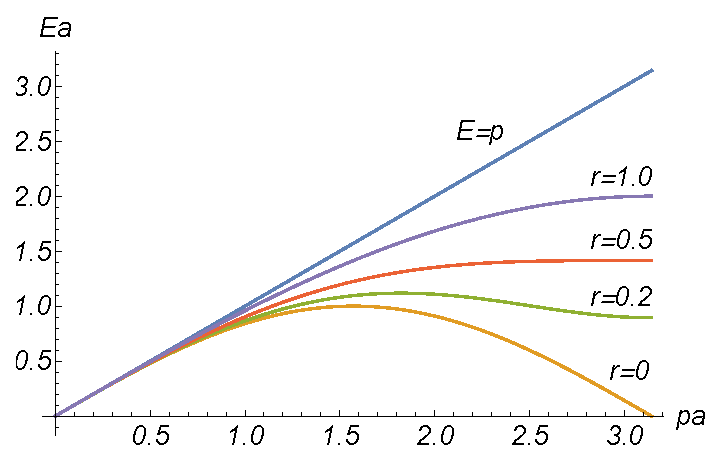
\includegraphics[scale=0.75]{Chapter3-figures/dispersion.eps}
 \end{center}
\caption{The  dispersion relation for massless fermion in (1+1)-dimension on the lattice for different values of 
 the Wilson's parameter $r$.  The linear dispersion in the continuum ($E=p$) is also shown for comparison.}
\label{fig:dispersion}
\end{figure}
%%%%%%%%%%%%%%%%%%%%%%%%%%%%%% 
 
 In general, $r\neq 0$  leads to a mass splitting   of 16 fermions:
$    m(p)  \simeq  m(0)\  (^{\forall }p_{\mu} \rightarrow 0) $ and 
$m(p)= m(0) +  \frac{2r}{a}N_{\pi}  \   (^{\exists }p_{\mu} \rightarrow \pi/a) $,
 where $N_{\pi}(=1,2,3,4)$ being the number of $\pi$'s
 in  $p_{\mu}a$.  This implies that we can select only one light
 fermion by choosing $m(0) \simeq 0$ and all the other
 15 fermions have masses of $O(1/a) $  for positive  $r$.  
 A price to pay  is that the non-vanishing  $r$ breaks chiral symmetry
 explicitly for finite $a$, i.e. $\{ \gamma_5, D_{\rm W} \} \neq 0$ even for $m(0)=0$.   
  Namely, the Nielsen-Ninomiya's no-go theorem is evaded by breaking the condition (v).

  Better way to  evade the no-go theorem 
  is to break the condition (v)  in a way that the definition of
 chiral symmetry is modified.  
 Suppose we consider a modified chiral rotation in the flavor space,
 \beq
 \label{eq:5.mod-chiral}
 q \rightarrow   {\rm e}^{-i \theta_{\rm {_A}} \hat{\Gamma}_5   } q, 
  \ \ \bar{q} \rightarrow \bar{q} {\rm e}^{-i \theta_{\rm {_A}} \Gamma_5 }  \ \ 
   {\rm with} \ \  \hat{\Gamma}_5 =  \Gamma_5 (1-2 a D_{_{\rm GW}})  ,
\eeq
which  reduces to the standard axial rotation for $a\rightarrow 0$.
Here  $D_{\rm GW}$ is a generalized Dirac operator which is 
 constructed so that   
  $\bar{q} D_{\rm GW} q$ is  invariant under
 Eq.(\ref{eq:5.mod-chiral}) even for finite $a$;
\beq
 \label{eq:5.GW-1}
\Gamma_5 D_{\rm GW} + D_{\rm GW} \hat{\Gamma}_5 =0 ,
\eeq
or equivalently  $\{ \Gamma_5, D_{_{\rm GW}} \} 
 = 2a D_{_{\rm GW}} \Gamma_5 D_{_{\rm GW}}$.
 This     is called the Ginsparg-Wilson relation.
  An explicit form of $D_{\rm GW}$ may be constructed as
\beq
 \label{eq:5.overlap-op}
 D_{\rm GW} = 
 \frac{1}{2a} \left( 1+  \frac{X}{\sqrt{X^{\dagger}X}} \right)  \ \  
 {\rm with} \ \ 
 X \equiv   D_{\rm W}^{(r=1)} - m_0  ,
\eeq
where $m_0 a$ being a dimensionless parameter of $O(1)$.
 Unlike the case of $m$ in the Wilson fermion,
 $m_0$  is not directly related to the physical fermion mass.
 Nevertheless,  if we choose the region $0< m_0 a < 2$,  
  there exists
 an  exact massless mode for $N_{\pi}=0$ for finite $a$,
 and  other 15 modes have a large mass 
 $(2/a)(2N_{\pi}-m_0 a)>0$.   (Exercise  \ref{prob:5}).
 
 Going back to the Wilson's fermion action, Eq.(\ref{eq:5.wilson-fermion}).
it  can be  conveniently rewritten  as 
\beq
 \label{eq:5.wilson-fermion-lat}
S_{\rm F}    
    & = & \sum_{n',n} \bar{\psi}(n') F(n',n;U) \psi(n) ,\\
\label{eq:5.wilson-fermion-op}
F(n',n;U) &=& \delta_{n'n} 
- \kappa \sum_{\pm \mu} \delta_{n',n+\hat{\mu}}
 (r + {\Gamma}_{\mu}) U_{\mu}(n),
\eeq
where we have redefined the quark field 
 as $\psi = a^{3/2} q /\sqrt{2\kappa }$ with
 $\kappa = [2(ma + 4r)]^{-1}$
 being the  {\it hopping parameter}. 
  If the quark mass $m$ is large, $\kappa$ is
 small and the ``hopping" to the 
  neighboring lattice site is suppressed.
   
%=================================
\subsection{Partition function on the lattice}
%=================================

The functional integration over quarks and gluons in continuum QCD
in Eq.(\ref{eq:Z-QCD}) is now transformed to the integration over quarks 
  on each site and gluons on each link in lattice QCD. 
 With Eq.(\ref{eq:5.wilson-action-cont}) and
   Eq.(\ref{eq:5.wilson-fermion-lat}), the partition function without the external field ($J=0$) reads
\beq
\label{eq:5.lattice-Z}
{\cal Z}  =  \int[dU d\bar{\psi}d\psi]   {\rm e}^{-  S_{\rm G}(U) - S_{\rm F}(\bar{\psi},\psi,U) }  
    =  \int[dU]\ {\rm Det}\ F(U) \ {\rm e}^{- S_{\rm G}(U) }
    = \int[dU]\  \ {\rm e}^{- S_{\rm eff}(U) }
\eeq
To obtain the second equality, we have explicitly carried out the integration over the
 Grassmann variables, $\bar{\psi}$ and $\psi$, 
 by using the formula in Appendix [Gaussian and Grassmann integrals]. Here ${\rm Det}$ implies the determinant in 
  spacetime, color, flavor and spin degrees of freedom.
In the third equality, the exponent  is defined as 
 \beq
\label{eq:Seff}
 S_{\rm eff}(U) \equiv S_{\rm G}(U) - {\rm ln Det} F(U).
 \eeq
 
 The integration over the group element $[dU] = \prod_{\mu,n} dU_{\mu}(n) $ can be defined through 
  the {\it Haar measure} $dU$ which has the property,
  $ d(V_{\rm L}U V_{\rm R}^{\dagger})=dU$
  with  $V_{\rm L,R}$ being arbitrary group elements. Such a measure is
   unique for compact groups such as SU$(N)$.
 If we parametrize the group element as $U=\exp(i \theta_a t^a)$,  one can define the 
 distance in the group space as $ds^2 = g_{ab}  (\theta) d\theta_a d\theta_b$, where the 
 metric is given by $g_{ab}=  {\rm tr} (L_aL_b) =  {\rm tr} (R_a R_b) $ with 
 \beq
 \label{eq:LR-form}
 L_a= -i U^{-1} ( {\partial} U/{\partial \theta_a}), \ \ \ 
 R_a= -i ({\partial}U/{\partial \theta_a} ) U^{-1}.
 \eeq   
 Then the Haar measure can be   explicitly written as
  \beq
  \label{eq:Haar-measure}
   dU = {\cal N} \sqrt{ \det g} \ \prod_a d\theta_a,
  \eeq
  with an overall normalization factor ${\cal N}$.
  
 The followings are some examples of the  SU($N$)  group integration, which can be proved
 by the invariant property of the Haar measure (except for the first one which determines the 
 normalization of the measure) (Exercise \ref{prob:6}):
 \beq
 \label{eq:group-int-0}
  & &   \int dU \  1  =  1 , \\ 
 \label{eq:group-int-1}
 & &   \int dU \ U_{ij}  =  0, \\
 \label{eq:group-int-2}
 & &    \int  dU \ U_{ij} U_{k\ell}^{\dagger}  =  \frac{1}{N} \delta_{i\ell} \delta_{jk} , \\
 \label{eq:group-int-4}
 & &  \int dU \ U_{ij} U_{k\ell}  U_{i'j'}^{\dagger} U_{k'\ell'}^{\dagger}
 = \frac{ \delta_{ij'} \delta_{ji'} \delta_{k\ell'} \delta_{\ell k'} + {(j' \leftrightarrow \ell',  i' \leftrightarrow k' ) }}{N^2-1}
   -  \frac{\delta_{ij'} \delta_{jk'} \delta_{k\ell'} \delta_{\ell i'} + { (j' \leftrightarrow \ell',  i' \leftrightarrow k' )}  }{N}, \\
 \label{eq:group-int-B}
 & &  \int dU \ U_{i_1 j_1} \cdots U_{i_N j_N} = 
 \frac{1}{N!} \epsilon_{i_1 \cdots i_N}    \epsilon_{j_1 \cdots j_N} .
 \eeq    

   
Similar to the statistical systems such as the Ising model, 
 observables are obtained by averaging over the statistical weight  as
 \beq
 \langle {\cal O} \rangle = \frac{1}{{\cal Z}}  \int[dU]\ {\cal O}(U) \ {\rm e}^{- S_{\rm eff}(U) }.
 \eeq
    Due to the gauge invariance of the Haar  measure,
 gauge non-invariant quantities have vanishing expectation values
  (Elitzer's theorem).  For example, consider the expectation value of the link variable,
 \beq
 \label{eq:elitzer}
 \langle U_{\mu} (n) \rangle 
 = \frac{1}{{\cal Z}}  \int [dU] U_{\mu} (n)  \ {\rm e}^{- S_{\rm eff}(U) }  = V(n)  \langle U_{\mu} (n) \rangle ,
\eeq
where we have made a change of variable, $U_{\mu}(n) \rightarrow V(n) U_{\mu}(n)$ with $V(n)$ 
being the $SU(N)$ matrix, and used the  gauge invariance of the Haar measure as well as ${\rm Det}\ F(U)$ and 
$S_{\rm G}(U)$.  Since Eq.(\ref{eq:elitzer}) must be true for arbitrary $V(n)$, we have $ \langle U_{\mu} (n) \rangle =0$.
 
Some examples of the non-vanishing  observables are shown  in Fig.\ref{fig:correlation}:
 (a) and (b) correspond to the mesic and baryonic correlations, respectively,  while (c) is a correlation related to the 
baryon-baryon interactions.  The filled circles are the spacetime points where the quarks and anti-quarks
are created or absorbed. Each  line with arrow indicates the quark propagator $F^{-1}(n,n';U)$ 
connecting two spacetime points $n$ and $n'$.  Thus, the explicit forms of the
 mesic and baryonic correlations are
 \beq
 \label{eq:correlation-M}
C_{\rm M}(n,n') 
 &=& \frac{1}{{\cal Z}}  \int [dU] \ F_{\alpha \beta}^{-1}(n,n';U) F_{\beta \alpha}^{-1}(n',n;U)  \ {\rm e}^{- S_{\rm eff}(U) } ,\\
\label{eq:correlation-B}
C_{\rm B}(n,n') 
 &=& \frac{1}{{\cal Z}}  \int [dU] \ \epsilon_{\alpha \beta \gamma} \epsilon_{\alpha' \beta' \gamma'} 
 F_{\alpha \alpha'}^{-1}(n,n';U) F_{\beta \beta'}^{-1}(n,n';U) F_{\gamma \gamma'}^{-1}(n,n';U)  \ {\rm e}^{- S_{\rm eff}(U) } ,
  \eeq
where all the color indices are contracted so that $C_{\rm M}$ and $C_{\rm B}$ are gauge invariant. 
 Other quantum numbers such as spin and flavor  associated with $F^{-1}$ are
 not shown explicitly.
  Spacetime, spin and flavor dependences of  $C_{\rm M}(n,n')$ in (a) and $C_{\rm B}(n,n')$ in (b)
  have all the information on the hadronic states in various different channels, while
  $C_{\rm BB}(n,m,n',m')$   in (c) has the information on baryon-baryon interactions.
      
% FIG %%%%%%%%%%%%%%%%%%%%%%%%%%
 \begin{figure}[t]
%\vspace{-1cm}
\begin{center}
%\framebox[74mm]{\rule[-26mm]{0mm}{52mm}}
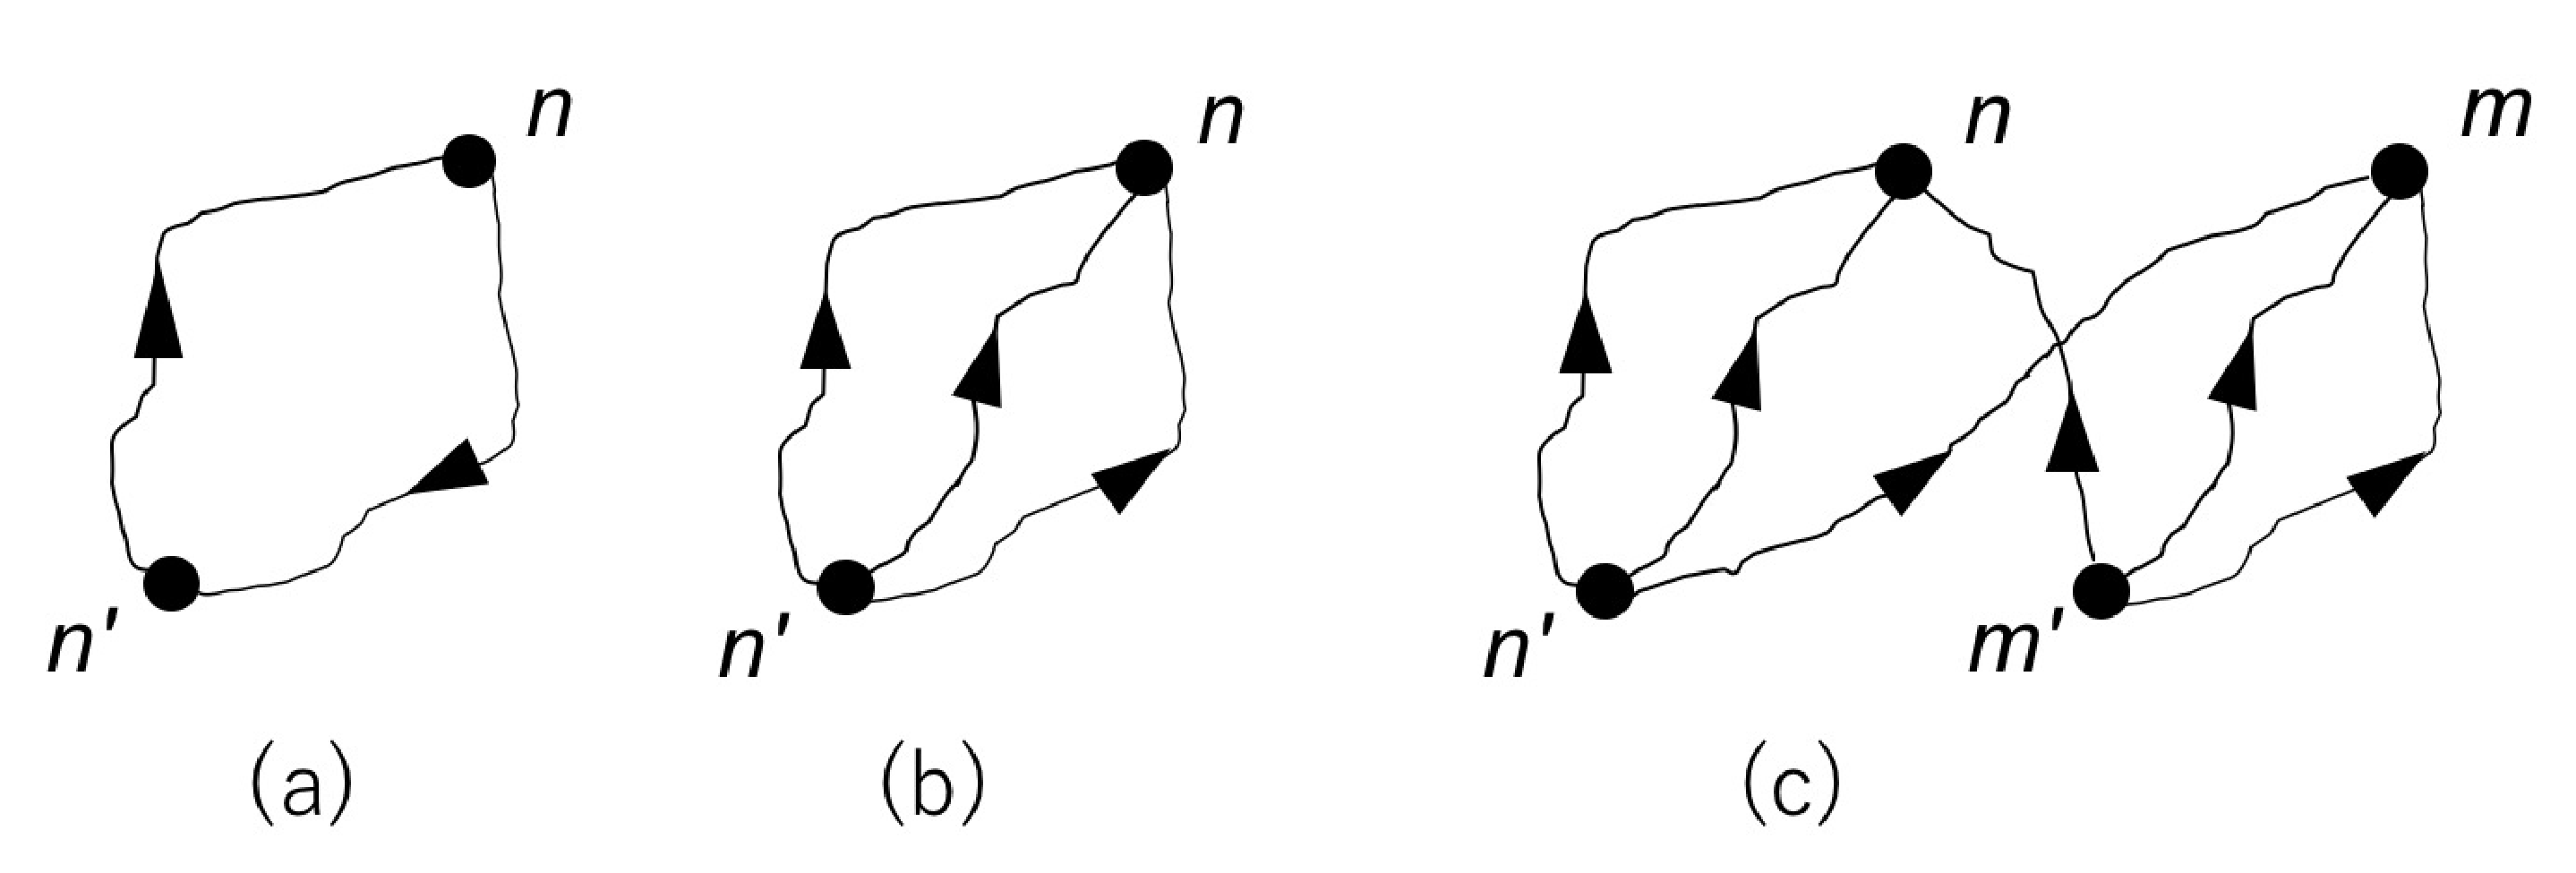
\includegraphics[scale=0.2]{Chapter3-figures/correlations.eps}
 \end{center}
%\vspace{-1cm}
\caption{
(a) Single meson correlation representing the propagation of a  meson created at point $n'$ and absorbed at point $n$.
(b)  Single baryonic correlation representing the propagation of a  baryon created at point $n'$ and absorbed at point $n$.
(c)  Two baryon correlation which contains the information on baryon-baryon interaction.}
\label{fig:correlation}
\end{figure}
%%%%%%%%%%%%%%%%%%%%%%%%%%%%%%%
 
   
%===========================================
\subsection{Strong coupling expansion and quark confinement}
%===========================================


% FIG %%%%%%%%%%%%%%%%%%%%%%%%%%
\begin{figure}[t]
\begin{center}
%\framebox[74mm]{\rule[-26mm]{0mm}{52mm}}
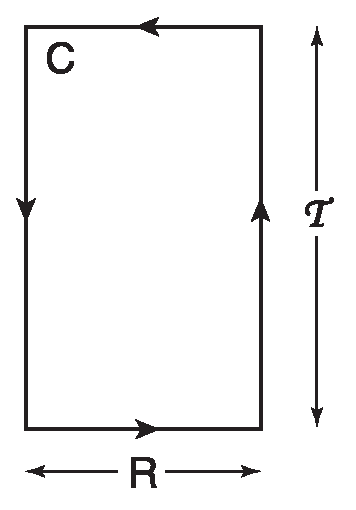
\includegraphics[scale=0.55]{Chapter3-figures/wilson-L.eps}
 \end{center}
\caption{A rectangular  Wilson loop with the
 temporal (spatial) size ${\cal T}$ ($R$).}
\label{fig:wilson-L}
\end{figure}
%%%%%%%%%%%%%%%%%%%%%%%%%%%%%%

One of the remarkable properties of QCD is the   confinement of quarks inside 
hadrons.  Simplest setup to see this phenomena is to consider
the potential $V(R)$ between  an infinitely heavy quark $Q$ and an anti-quark $\bar{Q}$ with
a fixed separation $R$.
It corresponds to Fig.\ref{fig:wilson-L} and can be written as
\beq
 \label{eq:5.wilson-loop-lattice}
\la W(C) \ra  
 & = & \la {\rm tr}\ \prod_{{\rm link}\in C}  U_{\mu}(n) \ra , \\
 \label{eq:5.wilson-loop-asym}
 & \propto  & 
  {\rm e}^{-V(R) {\cal T} } \simeq 
 \exp \left[ -\left( K R + b + \frac{c}{R} + \cdots \right) {\cal T} \right] ,
\eeq  
where we  have taken a limit     
${\cal T} \gg R \rightarrow \infty$ in   Eq.(\ref{eq:5.wilson-loop-asym}).
 Remembering the fact that the real time $t$ and the imaginary time $\tau$ are
 related as  $\tau=it$, the exponential falloff of  $\la W(C) \ra$ in $\tau$ implies the 
  temporal oscillation in $t$, and its $R$-dependent coefficient is nothing but the 
 interaction  energy between $Q$ and $\bar{Q}$.  
 
In Eq.(\ref{eq:5.wilson-loop-asym}), 
   $K > 0$  implies 
 the existence of a string-like
linear confining potential.
 It also implies 
 the area law  of the Wilson loop 
 $\la W(C) \ra \sim \exp(-K{\cal A})$
 where ${\cal A}= R \times {\cal T} $ is 
  the area inside the path $C$.
    In full QCD where pair creation of light quarks 
 are allowed,  
  the linear rising potential becomes eventually 
    flat at long distances due to the breaking of the string,
  $Q\bar{Q} \rightarrow (Q\bar{q})(q\bar{Q})$.
  
  To make the analysis simple, let us now consider the 
  SU$(N_c)$ Yang-Mills theory
  without light quarks: This is called the quenched 
  approximation and corresponds to take $F(U) =1$.
In this case,  the Wilson loop can be evaluated analytically
 in the strong coupling regime ($g \rightarrow \infty$).
First of all,  $S_{\rm G}$ is proportional to $1/g^2$,
so that  one can make an expansion,  
$\exp (-S_{\rm G}) = 1 - S_{\rm G}+ S_{\rm G}^2 /2 + \cdots $
 and finds (Exercise \ref{prob:7})
\beq
\label{eq:5.wilson-strong}
\la W(C) \ra = {1 \over {\cal Z}}
 \int [dU] \ {\rm tr} \prod_{{\rm link}\in C} U_{\mu}(n) \  
 \sum_{\ell =0}^{\infty} \frac{1}{\ell !} (-S_{\rm G})^{\ell}.
\eeq
 
Only the first three integrals, Eqs.(\ref{eq:group-int-0},\ref{eq:group-int-1},\ref{eq:group-int-2}),
 are necessary to extract the leading contribution to 
 $\la W(C) \ra $  in the strong coupling.
   Key observation is that all the $U$'s 
  from the Wilson loop and $U^{\dagger}$'s 
 from $(-S_{\rm G})^{\ell}$ should be paired in the leading order of $1/g^2$
 in   Eq.(\ref{eq:5.wilson-strong}).
  This means that the area inside the Wilson loop is tiled up 
 with minimum number of plaquettes as shown in
  Fig.\ref{fig:strong-c}. All the structures other than 
  the minimal surface are higher orders in  $1/g^2$.

% FIG %%%%%%%%%%%%%%%%%%%%%%%%%%
 \begin{figure}[t]
\begin{center}
%\framebox[74mm]{\rule[-26mm]{0mm}{52mm}}
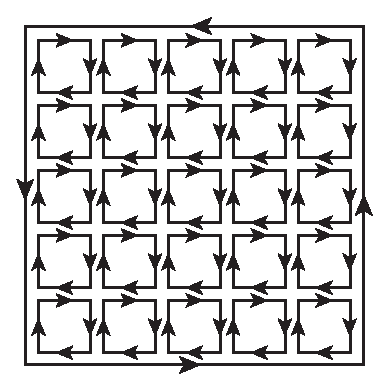
\includegraphics[scale=0.65]{Chapter3-figures/strong-c.eps}
 \end{center}
\caption{A minimum surface in which the Wilson loop is tiled 
   up by the fundamental plaquettes in the 
 strong coupling limit.}
\label{fig:strong-c}
\end{figure} 
%%%%%%%%%%%%%%%%%%%%%%%%%%%%%%

 In the evaluation of the numerator of
 Eq.(\ref{eq:5.wilson-strong}), 
 each plaquette has a contribution $1/g^2$. 
 Also each  integration on the link
   gives a factor $1/N_c$
   and the contraction of the color indices gives a factor $N_c$
 on each  site.
  On the other hand,
 ${\cal Z}$  (the denominator of Eq.(\ref{eq:5.wilson-strong})
 is   unity in the leading order. 
    Thus, one arrives at the formula in the lowest order
 of the strong coupling expansion,
\beq
 \label{eq:5.strong-estimate}
\frac{1}{N_c} \la W(C) \ra 
& & \xrightarrow[g^2\rightarrow \infty] 
 \  \frac{1}{N_c} \cdot  
\left(\frac{1}{g^2} \right)^{N_{\rm plaq}} \cdot  
\left(\frac{1}{N_c} \right)^{N_{\rm link}} \cdot N_c^{N_{\rm site}}  , \nonumber \\
& & \ \ \ \ \ \ \ \ \ \ \ =\left(\frac{1}{N_c g^2} \right)^{\frac{R {\cal T}}{a^2}} 
= \exp \left( - \frac{\ln N_c g^2}{a^2} R {\cal T} \right) ,
\eeq
where we have used a relation, $N_{\rm link}-N_{\rm site}+1 
 = N_{\rm plaq}$ and 
$N_{\rm plaq} a^2 = R {\cal T} ={\cal A}$.
 Since it shows the area law, \index{area law}
  the confinement is naturally obtained in the strong coupling
  with the linear rising potential, 
\beq
 \label{eq:5.linear-potential}
V(R) = K R \ \ {\rm with} \ \ K = \frac{1}{a^2} \ln (N_c g^2).
\eeq

 If we consider higher orders of the strong coupling expansion,
   ``rough" surfaces should be taken 
 into account.
 Nevertheless, the confining feature is
 stable against small perturbations in $1/g^2$.
  In fact, there exits a theorem 
  that,  for sufficiently large $g$, the strong coupling expansion 
  converges and shows confinement for all compact gauge groups  
  in all spacetime dimensions.
  

  A question here is that whether the real world 
  corresponds to the strong coupling region discussed above.
  The answer is no;  the real world corresponds to  the weak coupling regime. 
  For compact QED (quantum electrodynamics
  formulated in terms of the  U(1) link variable),
  the confinement  $K>0$ in the strong coupling regime 
   changes to  $K=0$ in the weak coupling regime.
  On the other hand,  in QCD in four spacetime dimensions 
 with $N_c=3$,   the confinement feature is expected to persist even in the weak coupling regime. 
 Indeed, there are  strong evidences for this statement 
  from  LQCD simulations.
  Its analytic proof, however,  is  still missing and is being one of the 
   most challenging problems in mathematical  physics.
   

%===============================================
\subsection{Weak coupling expansion and continuum limit}
%===============================================

  Lattice QCD can be regarded as an effective field theory
   with an ultraviolet (UV)  cutoff in the coordinate space. 
   The gauge coupling  $g$ is then interpreted as
  a bare coupling defined at the scale $a$ where
  quantum fluctuations with the wave length shorter than 
  $a$ are integrated out.  In non-Abelian gauge theories,
   it can be shown that $g(a)$ decreases logarithmically as $a$ decreases
   unless the number of matter fields is not too large.  
    This is called the {\it asymptotic freedom}, and is essential for taking
    the continuum limit ($a \rightarrow 0$) to remove the 
    lattice artifact. 
        
 For simplicity, let us consider the case with massless fermions, where 
 observables
   ${\cal O}$ such as the string tension and the hadron masses  depend only
   on the coupling $g$ and the  regularization scale $a$. 
   Then,  from the dimensional ground, one can  write  
     \beq
\label{eq:5.O-dim}
 {\cal O} (g(a),a) = a^{-d} X(g(a)),
 \eeq
 where $d$ is the mass-dimension of ${\cal O}$ and $X$ is a dimensionless
 function of $g$.  The $a$-independence of the observable implies
 \beq
\label{eq:5.O-RG}
 a{d{\cal O} \over da} 
  =  
  \left( a \frac{\partial}{\partial a} 
 - \beta_{_{\rm LAT}}  \frac{\partial}{\partial g} \right) {\cal O}(g(a), a)  = 0 , 
\ \   \beta_{_{\rm LAT}}(g) =  -a {dg(a) \over da} .
\eeq
By integrating the first equation in Eq.(\ref{eq:5.O-RG}),  we find
\beq
\label{eq:5.lat-F}
 X(g) = 
 \exp \left( -d \int^g {dg' \over \beta_{_{\rm LAT}}(g')} \right) .
 \eeq
Suppose that 
 the beta-function can be expanded in terms of $g$ for small $a$:
$\beta_{_{\rm LAT}}(g)   = 
  - \beta_0 g^3 - \beta_1  g^5 + \cdot \cdot \cdot $. Here
  $\beta_0$ and $\beta_1$ can be shown to be independent of the 
   regularization scheme and are known to be 
\beq
\beta_0= \frac{1}{(4\pi)^2} \left( \frac{11N_c}{3}-\frac{2N_f}{3} \right),
\ \ \  \beta_1= \frac{1}{(4\pi)^4} \left( \frac{34N_c^2}{3}-\frac{38N_f}{3} \right),
\eeq
           for QCD with $N_c$ colors and     $N_f$ fermions.
  
% FIG %%%%%%%%%%%%%%%%%%%%%%%%%%
 \begin{figure}[t]
\begin{center}
%\framebox[74mm]{\rule[-26mm]{0mm}{52mm}}
%\includegraphics[scale=0.6]{as-scale.eps}
\includegraphics[scale=0.30]{Chapter3-figures/crossover.eps} 
 \end{center}
\caption{Crossover behavior of the dimensionless
 string tension $Ka^2$ from the strong coupling
 regime  $\beta=2N_c/g^2 \rightarrow 0$ to the weak coupling
  (asymptotic scaling) regime  $\beta=2N_c/g^2 \rightarrow \infty$
  for SU($N_c=2$) Yang-Mills theory.  The figure is adapted from
  \cite{Creutz:1980zw}.
  }
\label{fig:as-scale}
\end{figure}
%%%%%%%%%%%%%%%%%%%%%%%%%%%%%%%%

        
By integrating  the second equation in Eq.(\ref{eq:5.O-RG}) with the above expansion of
$\beta_{_{\rm LAT}}(g)$, one finds  
 \beq
\label{eq:5.a-vs-L}
 a = \Lambda_{_{\rm LAT}}^{-1} \cdot  
 \exp  \left( -\frac{1}{2\beta_0 g^2}  \right)  \cdot
  (\beta_0 g^2)^{-{\beta_1 \over 2 \beta_0^2}} 
 \cdot (1 + O(g^2)).
 \eeq
Here  $\Lamlat$ is called the scale parameter on the lattice, and  
   $g(a)$ can be expressed in terms of $a$ and $\Lamlat$ ((Exercise \ref{prob:8}),
 \beq
\label{eq:5.lat-running-g}
{1 \over g^2(a)} = \beta_0 \ln \left( 1 \over a^2 \Lamlat^2 \right)
+ {\beta_1 \over \beta_0} \ln \ln \left( 1 \over a^2 \Lamlat^2 \right)
+ \cdot \cdot \cdot .
\eeq
 This is the asymptotic freedom
 in which $g(a)$ decreases as $a$ decreases.  This also justified the 
 assumption that the beta-function can be expanded by $g(a)$ for small $a$.
 
 
Direct way to extract the actual value of $\Lamlat$  is to
 carry out  numerical simulations of  
 a certain physical quantity (such as the string tension)
 and compare the result with the experimental value. 
 For example, the string tension, which has mass-dimension
 two ($d=2$) should  behave as
\beq
\label{eq:5.lat-K}
K a^2 = C_K \exp \left( - {1 \over \beta_0 g^2} \right) 
(\beta_0 g^2)^{-\beta_1 /\beta_0^2} = C_K \Lamlat^2 ,
\eeq
with $C_K$ being a dimensionless numerical constant independent
 of $g$.  As  can be seen from this example, 
 the functional form of the physical quantities 
 for $g\sim 0$  is  severely constrained.  
This is called the {\em asymptotic scaling} which 
 is used to check whether the system is 
  close enough to the continuum limit.
Shown in Fig.\ref{fig:as-scale} is a historic numerical study, which shows 
 a crossover of $Ka^2$  from the strong coupling regime to the weak coupling regime
 in SU(2) Yangs-Mills theory. 
  


%===============================
\subsection{Running coupling}
%===============================

% FIG %%%%%%%%%%%%%%%%%%%%%%%%%%
\begin{figure}[t]
\begin{center}
%\framebox[74mm]{\rule[-26mm]{0mm}{52mm}}
%\includegraphics[scale=0.6]{as-scale.eps}
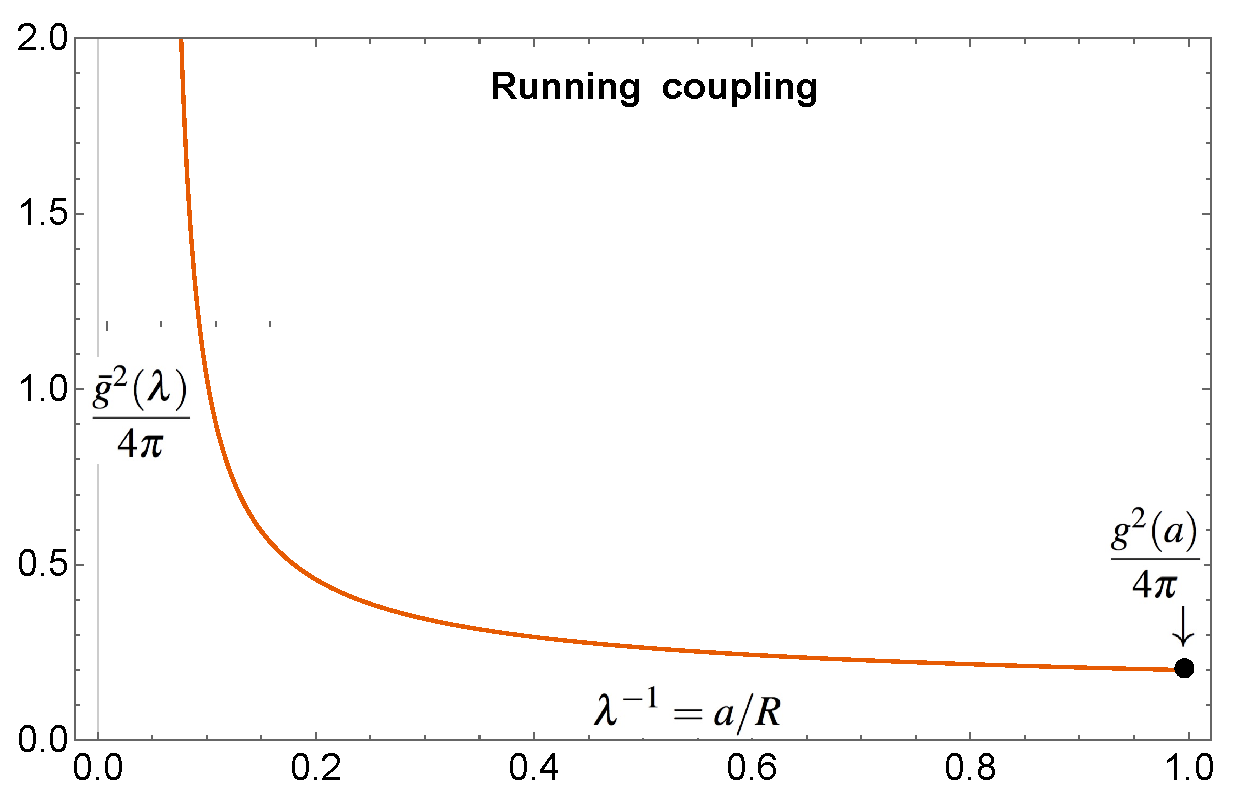
\includegraphics[scale=0.45]{Chapter3-figures/running-g.eps} 
 \end{center}
\caption{Perturbative running coupling $\frac{1}{4\pi}\bar{g}^2(\lambda)$ as a function of $\lambda^{-1}$.
In the short distance limit ($\lambda =1$), the running coupling coincides with the bare coupling $\bar{g}(\lambda=1)=g(a)$,
while, in the long distance regime ($\lambda \ll 1$), the running coupling grows. }
\label{fig:running-g}
\end{figure}
%%%%%%%%%%%%%%%%%%%%%%%%%%%%%%%


Let us now consider an observable ${\cal O}$ which depends 
not only on $g(a)$ and $a$ but also on some external dimensionful parameter.
For concreteness, we consider the heavy quark potential $V(R; g(a),a)$ in the 
quenched approximation.  Since it has the dimension of energy, one may write
\beq
V(R,g(a),a) = R^{-1} \tilde{V} (R/a, g(a)).
\eeq
Then the cutoff independence of the observable, $a \frac{d}{da}V(R,g(a),a)=0$,  leads to
\beq
\left( \lambda \frac{\partial}{\partial \lambda} + \beta_{_{\rm LAT}} \frac{\partial}{\partial g} \right) \tilde{V} (\lambda,g)=0,
\label{eq:RG-R}
\eeq
where we have introduced 
a dimensionless  scaling parameter $\lambda$ through $R=\lambda a$.

]The solution of the {\it renormalization group equation}, Eq.(\ref{eq:RG-R}), reads
\beq
\label{eq:RG-sol}
 \tilde{V} (\lambda,g(a)) = \tilde{V} (1, \bar{g}(\lambda)).
 \eeq
 Here $\bar{g}(\lambda)$ is called the {\it running coupling} which is  a solution of
\beq
\lambda \frac{d\bar{g}}{d\lambda}  = - \beta_{_{\rm LAT}} (\bar{g}(\lambda)),
\eeq
with the boundary condition, $\bar{g}(\lambda=1)= g(a)$.
One can show that  Eq.(\ref{eq:RG-sol})  satisfies Eq.(\ref{eq:RG-R}) explicitly by applying the partial derivatives 
 or more generally by the method of characteristics in Appendix [Method of characteristics].
Then, we eventually arrive at the formula 
\beq
V(R,g(a), a) = \frac{a}{R} V (a, \bar{g}(R/a), a) .
\eeq
If $R$ is  in the interval,  $a < R \ll \Lamlat^{-1}$, the running coupling $\bar{g}$ is small enough, so that 
one may use the perturbative expansion of $\beta_{_{\rm LAT}}$ to obtain
\beq
\bar{g}^2(R/a) \simeq \frac{g^2(a)}{1-2\beta_0 g^2(a) \ln (R/a)} =  \frac{1}{2\beta_0 \ln (1/(R\Lamlat) ) }. 
\label{eq:running-R}
\eeq 
In Fig.\ref{fig:running-g}, the behavior of $\frac{1}{4\pi}\bar{g}^2(\lambda)$  as a function of $\lambda^{-1}$ is shown.
The bare coupling $\frac{1}{4\pi}g^2(a)$ appears as the boundary condition at shortest distance $\lambda=R/a=1$,
while $\frac{1}{4\pi} \bar{g}^2(\lambda)$ grows  as $\lambda$ increases.
The latter implies that the strong interaction has anti-screening feature.

For $R$ sufficiently close to $a$, one may evaluate the potential by using perturbation theory as
$V (a, \bar{g}(R/a), a)  = - C_{{\rm F}} \frac{\bar{g}(R/a)^2}{4\pi a}$, so that we finally obtain
\beq
\label{eq:RG-Coulomb}
V(R,g(a),a) \simeq - C_{{\rm F}} \frac{\bar{g}^2(R/a)}{4\pi R} \ \ \ \ \ (a < R \ll \Lamlat^{-1}),
\eeq
where $C_{{\rm F}}=4/3$ for $N_c=3$ is given in Appendix [SU($N$) algebra].
Eq.(\ref{eq:RG-Coulomb}) is nothing but the Coulomb potential with the running coupling constant.
Note that the left hand side is $a$-independent, while the right hand side has
logarithmic $a$-dependence through $\bar{g}$.  This is due to the use of perturbation theory;
such a logarithmic $a$-dependence  is cancelled by the next-to-leading order term.
Note also that the similar analysis can be done for any other observables.
The QCD thermal pressure at finite temperature $P(T,g(a),a)$ is a typical example, in which 
the weak coupling analysis (i.e. the description by  quark-gluon plasma picture)
is justified  under the condition  $ \Lamlat \ll T < a^{-1}$. 



%%%%%%%%%%%%%%%%%%%
\section{Lattice QCD:  numerical simulations}
%%%%%%%%%%%%%%%%%%%


Suppose we have a lattice having $\Ns$ ($\Ntau$) number of sites
in each spatial (temporal) direction. Then 
 the total number of links is 
   $  \Ns^3 \times \Ntau  \times 4$. 
 Therefore the total  number of gluon integrations $\int [dU]$
 for a moderate lattice size  $\Ns = \Ntau =32$ reads
\beq
\label{eq:5.lattice-size}
 ( \Ns^3 \times \Ntau \times 4 )_{\rm links} \times 8_{\rm color} 
 \sim 3 \times 10^7 .
 \eeq
 This is 
 hopelessly a large number  
  for standard methods of numerical integration。
   In this case,  the  Monte Carlo (MC) integration,
   which is a
  statistical way to evaluate the integral, plays a 
   powerful role. For rapidly varying integrand,
  the MC integration should be supplemented by the 
 importance sampling 
   to have better accuracy, in which the rapidly varying
   part is sampled more than the slowly varying part.
     
     
 %==========================
\subsection{Importance sampling}
\label{ss:IS}
%==========================
    
     Let us consider the general partition function ${\cal Z}= \int [d\phi] \exp(-S(\phi)) $,
    with some c-number field $\phi$  and try to calculate  an observable ${\cal O} $ by
  \beq
  \langle {\cal O} \rangle = \frac{1}{{\cal Z}} \int [d \phi] \ {\cal O} (\phi) e^{-S(\phi)}.
  \eeq   
  The basic procedure of the MC integration
  with the {\it importance sampling} consists of two steps:
  \begin{enumerate}
  \item[(I)]   Generate a set of field configurations, $ \{  \phi^{(1)}, \phi^{(2)}, \cdots, \phi^{(N)} \}$, 
with $\phi^{(n)}$  being arranged to appear with 
 a probability in ``equilibrium", $W_{\rm eq}[\phi]={\cal Z}^{-1} \exp (-S(\phi))$.
 \item[(II)]  The field configurations thus generated 
 are  used to calculate the expectation value,
 \beq
\label{eq:5.obs-average}
\la {\cal O} \ra = \frac{1}{N}\sum_{n=1}^N {\cal O}^{(n)}
\pm \sqrt{{\sigma^2 \over N}}, \ \ \ \ \ 
\sigma^2 =  \frac{1}{N-1} \sum_{n=1}^N \la {\cal O}^{(n)} - \la {\cal O} \ra \ra^2 ,
\eeq
with ${\cal O}^{(n)}={\cal O}(\phi^{(n)})$.
\end{enumerate}

 %=========================================
\subsection{Markov chain Monte Carlo (MCMC)}
%==========================================
  
 For large  number of integration variables such as Eq.(\ref{eq:5.lattice-size}), 
 it  is essential to develop an appropriate scheme to carry out  Step (I) in Sec. \ref{ss:IS}. 
 The {\it Markov chain Monte Carlo (MCMC)}  method is one of such schemes. 
    
Let us consider a chain of configurations  generated successively starting from an
initial configuration,
\beq
\label{eq:M-chain}
 \phi_{0} \rightarrow  \phi_{1} \rightarrow \phi_{2}
 \rightarrow \cdots \rightarrow \phi_{i} \rightarrow  \phi_{i+1}
\rightarrow \cdots ,  
\eeq
where the ``{\it update}" of the $i$-th configuration ($\phi$)  to
the $(i+1)$-th configulation ($\phi'$)  is governed by the conditional probability
$P$ or equivalently  the transition matrix $\vT$, 
\beq
\label{eq:M-transition}
P(\phi \rightarrow \phi') = (\vT)_{\phi \phi'} 
\eeq
which has the property, $\sum_{\phi'} P(\phi \rightarrow \phi')=1$.
Eq.(\ref{eq:M-chain}) generated by Eq.(\ref{eq:M-transition}) is called the {\it Markov chain} since
it is governed by the Markov process where the conditional probability depends only on the 
neighbouring pair. The probability distribution $W[\phi]$ (with the properties, $W[\phi] \ge 0$ and 
$\sum_{\phi} W[\phi]=1$) is updated successively by Eq.(\ref{eq:M-transition}),
\beq
\label{eq:5.MC-update}
W'[\phi' ] =  \sum_\phi  W[\phi] P(\phi \rightarrow \phi'). 
\eeq

If  the Markov chain is {\it irreducible} (any $\phi$ and $\phi'$ are connected with each other) and  {\it aperiodic}
(absence of $\phi$ which appears periodically) \footnote{Rigorous definitions are as follows. (i) The Markov chain is said to be 
irreducible if one can find a finite positive integer $n (< \infty)$  such that  $(\vT^n)_{\phi \phi'} > 0 $ for all $\phi$ and $\phi'$.
(ii)  The period, $d(\phi)$, is defined by the greatest common divisor  of the set of positive integers $n (\ge 1)$
such that  $(\vT^n)_{\phi \phi} > 0 $ is satisfied. If $d(\phi)=1$ for all $\phi$, the Markov chain is 
said to be aperiodic \cite{Haggstrom:2002}.},  there exists a theorem that the Markov chain
 has a unique equilibrium distribution $W_{\rm eq}$ satisfying 
\beq
\label{eq:transition-W}
W_{\rm eq}[\phi']  =  \sum_\phi W_{\rm eq}[\phi] P (\phi \rightarrow \phi'),
\eeq
and it can be reached by $\vT^{\infty}$ starting from arbitrary initial distribution.
For a heuristic proof of this theorem, see Exercise \ref{prob:9}. For mathematical proof,  see  \cite{Haggstrom:2002}.

As is easily seen, a  sufficient but not necessary condition for $P$ to lead $W_{\rm eq}$  is the {\it detailed balance}:
\beq
\label{eq:5.det-balance}
W_{\rm eq}[\phi] P (\phi \rightarrow \phi' )  =
 W_{\rm eq}[\phi'] P (\phi' \rightarrow \phi ).
\eeq
There also exits specific algorithm without the detailed balance in MCMC  \cite{SuwaTodo:2010}.


The Markov chain Eq.(\ref{eq:M-chain})  takes 
certain {\it thermalization time} to reach equilibration. 
Also, the nearby  field configurations  are strongly correlated  during the {\it autocorrelation time}.
To calculate the actual average in Eq.(\ref{eq:5.obs-average}), we then 
need to discard non-themalized configurations and also 
thin out the configurations to avoid the autocorrelations. 
This is schematically shown for an observable ${\cal O}$ in Fig.\ref{fig:auto}.
The thermalization time can be estimated by monitoring the behavior of ${\cal O}$  under 
successive update, while the autocorrelation time can be estimated by 
calculating the correlations of ${\cal O}$ for different configurations.

 
% FIG %%%%%%%%%%%%%%%%%%%%%%%%%%
\begin{figure}[t]
\begin{center}
%\framebox[74mm]{\rule[-26mm]{0mm}{52mm}}
%\includegraphics[scale=0.6]{as-scale.eps}
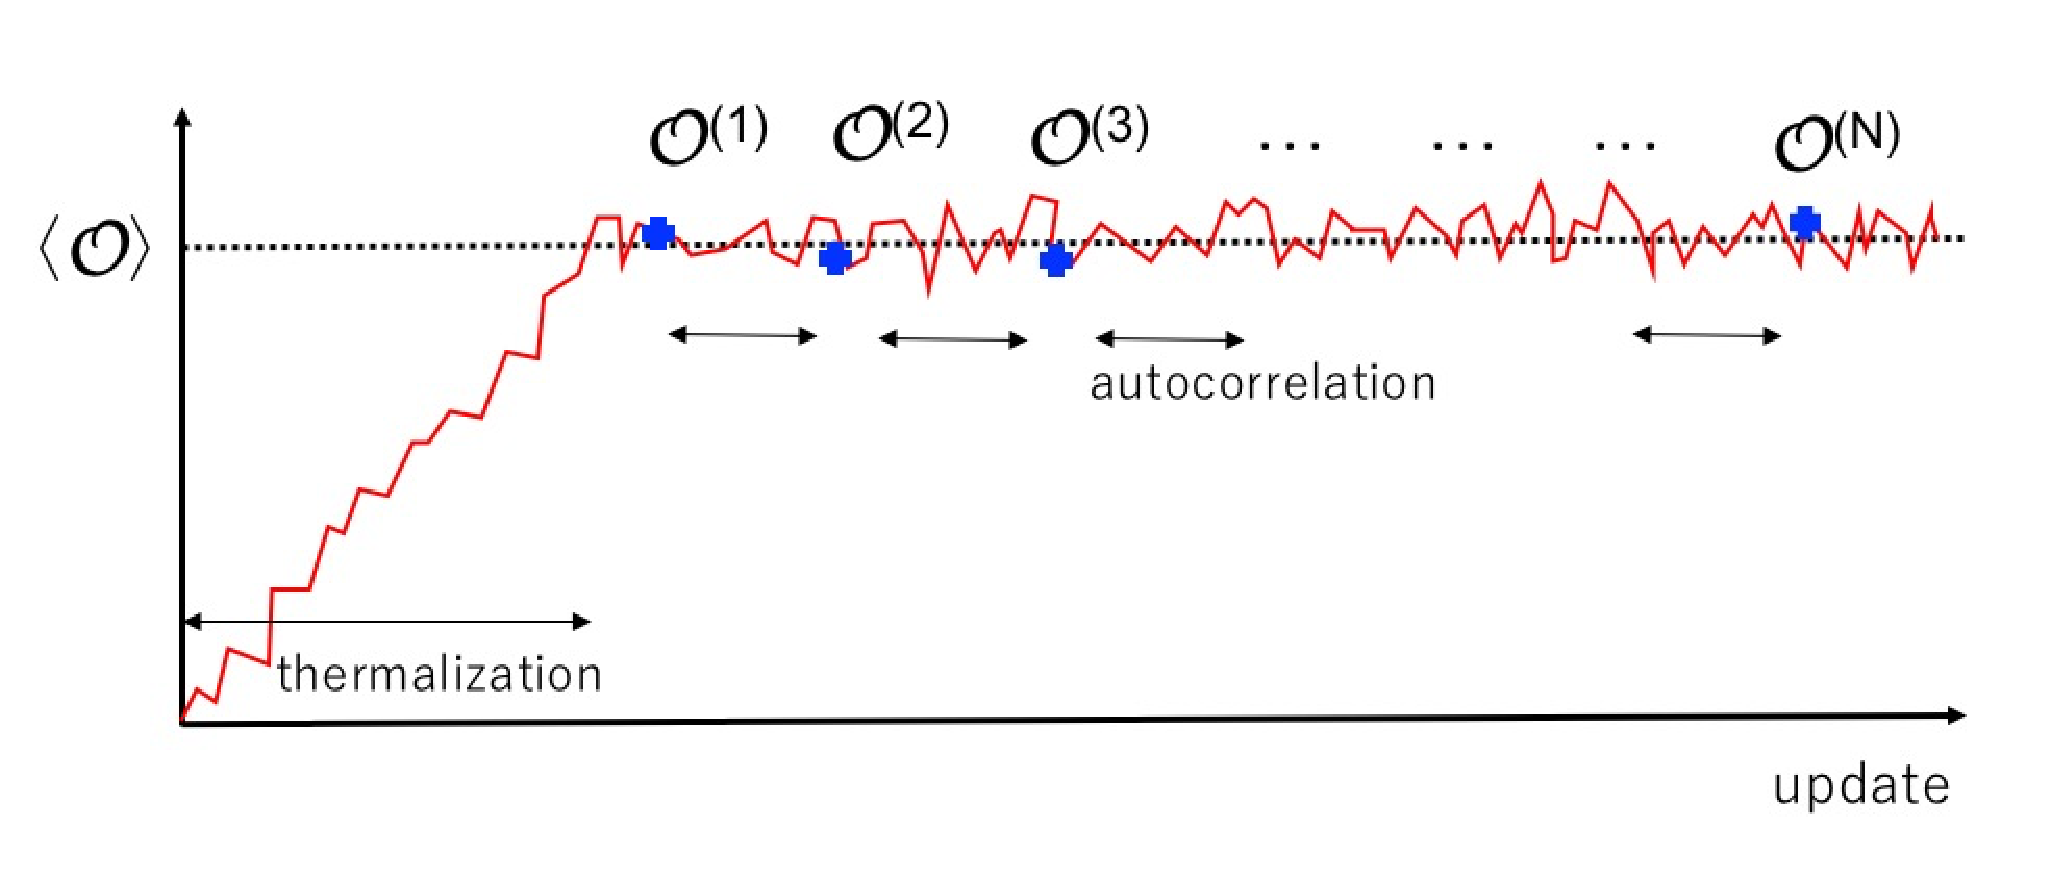
\includegraphics[scale=0.37]{Chapter3-figures/auto.eps} 
 \end{center}
\caption{Schematic illustration on the behavior of ${\cal O}$ under successive update starting from
certain initial configuration. Blue crosses correspond to ${\cal O}^{(n)}$ to be used for the actual average in
Eq.(\ref{eq:5.obs-average}).}
\label{fig:auto}
\end{figure}
%%%%%%%%%%%%%%%%%%%%%%%%%%%%%%
    
    
    
%===============================
\subsection{Hybrid Monte Carlo (HMC)}
%===============================

 Most widely used method   for 
  generating configurations in LQCD 
  is  the hybrid Monte Carlo (HMC) method \cite{Duane:1987de} and its variations.
 The basic procedure of the HMC can be summarized as follows:
 First, we rewrite the partition function by introducing a conjugate momentum field $\pi$,
 so that ${\cal Z}$ is transformed to a phase space functional integral,
\beq
{\cal Z}= \int [d\phi]\ e^{-S(\phi)}= \int [d\Phi] \  e^{- H(\Phi)}, \ \  \ \ \ 
H(\Phi) = \frac{1}{2} \pi^2 + S(\phi) ,
\eeq
where $\Phi\equiv(\phi,\pi)$ and $[d\Phi]\equiv [d\phi d\pi]$.
Then we follow the steps below:
 \begin{enumerate}
 \item[1.]   Start with arbitrary chosen initial configuration, $\phi$.
 \item[2.]  Generate $\pi$ with the Gaussian distribution, 
 \beq 
 P_{\rm G}(\pi) \propto \exp(-\pi^2/2).
 \eeq
\item[3.]  Evolve $\Phi $ under transition probability $P_{\rm H}$ with the {\it reversibility condition}, 
\beq
\label{eq:reversible}
P_{\rm H}(\Phi \rightarrow \Phi') = P_{\rm H}(\Phi'_r \rightarrow \Phi_r),   \ \ \  \Phi_r \equiv (\phi,-\pi). 
\eeq
\item[4.] Accept the configuration $\Phi'$ with the probability, 
\beq 
\label{eq:MET-test}
P_{\rm A} (\Phi \rightarrow \Phi')  = {\rm min.} \{ 1, e^{-\Delta H} \} ,
\eeq
where  $\Delta H=H(\Phi')- H(\Phi)$.  This is called the {\it Metropolis test}  \cite{Metropolis_1953}.
\item[5.] If the new configuration $\Phi'$ is accepted, go to Step 2 with $\phi'$.
 Otherwise, keep the original $\phi$ and go to Step 2. 
\end{enumerate}

The above procedure satisfies the detailed balance  Eq.(\ref{eq:5.det-balance}) 
with $W_{\rm eq}[\phi]=\exp(-S(\phi))$. 
In fact, the Step 4  satisfies the detail balance in phase space (Exercise \ref{prob:10}),
\beq
\label{eq:DT-balance}
e^{-H(\Phi)} P_{\rm A} (\Phi\rightarrow \Phi') = e^{-H(\Phi')} P_{\rm A} (\Phi' \rightarrow \Phi) .
\eeq
Then, we have
\beq
e^{-S(\phi)} P (\phi \rightarrow \phi' ) 
&=& e^{-S(\phi)} \int [d\pi d\pi'] P_{\rm G}(\pi)  P_{\rm H}(\Phi \rightarrow \Phi') P_{\rm A} (\Phi \rightarrow \Phi') , \nonumber \\
&=& \int [d\pi d\pi']\ e^{-H(\Phi)}  P_{\rm H}(\Phi \rightarrow \Phi') P_{\rm A} (\Phi \rightarrow \Phi') ,\nonumber \\
&=& \int [d\pi d\pi']\ e^{-H(\Phi')}  P_{\rm H}(\Phi \rightarrow \Phi') P_{\rm A} (\Phi' \rightarrow \Phi) ,\nonumber \\
&=& \int [d\pi d\pi']\ e^{-H(\Phi')}  P_{\rm H}(\Phi'_r \rightarrow \Phi_r)  P_{\rm A} (\Phi' \rightarrow \Phi) ,\nonumber \\
&=& \int [d\pi d\pi']\ e^{-H(\Phi')}  P_{\rm H}(\Phi' \rightarrow \Phi ) P_{\rm A} (\Phi' \rightarrow \Phi) ,\nonumber \\
&=& e^{-S(\phi')} \int [d\pi d\pi'] P_{\rm G}(\pi')  P_{\rm H}(\Phi' \rightarrow \Phi)  P_{\rm A} (\Phi' \rightarrow \Phi) 
= e^{-S(\phi')}  P (\phi' \rightarrow \phi ) ,
\eeq
where we have used Eq.(\ref{eq:reversible}) to obtain the 4th line, and also used $H(\Phi)=H(\Phi_r)$ 
 to obtain the 5th line. 

Note that $P_{\rm H}$ can be chosen to be any transition probability as long as it satisfies
Eq.(\ref{eq:reversible}).  In practice, the deterministic procedure based on the Molecular Dynamics (MD) 
evolution along the  ``computer"  time $s$ is useful:
\beq
\label{eq:MD}
\frac{d}{ds} 
\left(
\begin{array}{cc}
 \phi  \\
  \pi 
\end{array}
\right)
=
\left(
\begin{array}{cc}
 0 &  1   \\
 -1  & 0   
\end{array}
\right)
\left(
\begin{array}{cc}
  {\delta H (\phi,\pi)}/{\delta \phi}   \\
  {\delta H (\phi,\pi)}/{\delta \pi}
\end{array}
\right) =
\left(
\begin{array}{cc}
 \pi  \\
  -  {\delta S (\phi)}/{\delta \phi}
\end{array}
\right) ,
\eeq
which leads to
\beq
P_{\rm H}(\Phi \rightarrow \Phi')  = \delta (\Phi' - \Phi(s)),
\eeq
 on the phase space trajectories, $\Phi = \Phi(0) \rightarrow \Phi(s)$. 
 
If we do not introduce the MD before the Metropolis test $P_{\rm A}$, the procedure is essentially the MCMC
with the Metropolis test.  It becomes, however,
 very slow for non-local action such as Eq.(\ref{eq:Seff})
where $S_{\rm G}(U)$ is local in spacetime while ${\rm Ln Det} F(U)$ is non-local.
The MD is a nice way to evolve the whole variables on the lattice at once.
 The  computer time $s$ needs to be discretized with a step size $\varepsilon$,  which brings 
 inevitable numerical error in MD. However,   the Metropolis test in Step 4 eliminates such error so that
no extrapolation to $\epsilon$ is required in HMC.

 There are numerical algorithms in MD  to satisfy the reversibility and preserve the phase space area 
 exactly for finite $\varepsilon$.   The
  {\it leapfrog integrator} is one of such algorithms widely used in LQCD 
  (see Appendix [Leapfrog integrator in molecular dynamics]).
 Since this  conserves the Hamiltonian with $0(\varepsilon^2$) accuracy, the acceptance rate
 in Step 4 can be kept high.


 In LQCD simulations, we need to treat the unitary matrices $U_{\mu}(n)$ as dynamical variables, i.e.
  the MD should be performed on the SU($N_c$)  group manifold.
 The appropriate choice of the conjugate momentum would be the element of the Lie algebra,
  $ P_l =  R_l^a t^a = -i  (d{U_l}/ds) U_l^{-1} $ (see Eq.(\ref{eq:LR-form})) where
  we have abbreviated the link index $n$ and site index $\mu$  as $l$ for simplicity.
 This  leads to the
  equation of motion for $U_l$,
\beq
\label{eq:EOM-U}
\frac{d U_l}{ds}= i P_l U_l .  
\eeq
The effective Hamiltonian is naturally written as 
\beq
\label{eq:EOM-H}
H= {\rm tr} \sum_{l} P_l^2 + S_{\rm eff}(U) , 
\eeq
 where ${\rm tr}$ is over color indices with the normalization given in Eq.(\ref{eq:tt}).
 Then the  time-parameter independence  $\frac{dH}{ds}=0$ leads to the equation of motion for $P_l$
 (Exercise \ref{prob:11}),
  \beq
 \label{eq:EOM-P} 
 \frac{dP_l}{ds} = - i  \sum_{i,j} t^a \left( t^a U_l \right)_{ij} \frac{\partial S_{\rm eff}(U)}{\partial (U_l)_{ij}}.
\eeq
In the actual simulations, the ${\rm ln Det}F(U) $ part of the effective action is treated by
introducing a set of bosonic variables (pseudofermions) through the identity,
\beq
{\rm Det} F = ({\rm Det} F^{-1})^{-1} = \int [d\chi^* d\chi] \ \exp \left( -\sum_{IJ} \chi^*_{I} F_{IJ}^{-1} \chi_J \right),
\eeq
where $I$ and $J$ stand for all possible internal and spacetime indices carried by $F$.    
For further details of HMC (and its variations) with pseudofermions, 
consult the recent review \cite{Schaefer:2012tq} and references therein.


%===========================
\subsection{Error estimate}
%===========================

There are two kinds of errors  in the data obtained from  LQCD simulations.\\

\noindent {\bf Systematic errors:} \\
 They are related to the lattice spacing $a$, the lattice volume $L^3$,
  and the quark masses ($m$).  During 
  the continuum extrapolation ($a\rightarrow 0$) and the thermodynamic extrapolation ($L \rightarrow \infty$) 
  under the  guidance of  the asymptotic scaling for small $a$ 
 and the finite size scaling for  large $L$, some systematic errors are brought in.
 Also,  one often needs to make extrapolation to the physical quark mass by using 
 lattice data  with heavier  quark masses. This  also brings some
 systematic errors.\\
 
 \noindent
{\bf Statistical error:} \\
It originates from the importance sampling.  A very useful procedure to estimate such error
 commonly used in LQCD is the {\it jackknife resampling method}. (The name
  originates from the ``jackknife"  which is an easy and  portable  tool  for general purposes).
  Let us consider the mean and the unbiased variance of a certain quantity $ {\cal O}$,
  \beq
   \la {\cal O} \ra = \frac{1}{N} \sum_{n=1}^N {\cal O}^{(n)}  \pm \sqrt{\frac{\sigma^2({\cal O} )}{N}}, \ \ \ \
   \sigma^2({\cal O}) = \left( \frac{N}{N-1} \right)  \frac{1}{N} \sum_{n=1}^N ( {\cal O}^{(n)}  - \la {\cal O} \ra )^2,
  \eeq
where the factor $\frac{N}{N-1}$ is called the Bessel's correction.
 The jackknife samples are obtained by
 \beq
  {\cal O}^{(n)}_J= \frac{1}{N-1} \sum_{n' \neq n}  {\cal O}^{(n')}      \ \ \ \  (n=1, \cdots, N).
 \eeq
 If we need to make a quick estimate of the 
  mean and the variance of a function $f({\cal O})$, we have
 \beq
\label{eq:jack}
 \la f({\cal O}_J)\ra = \frac{1}{N} \sum_{n=1}^{N} f( {\cal O}^{(n)}_J) \pm  \sqrt{\frac{\sigma_J^2(f)}{N}}, \ \ \ \ 
  \sigma_J^2(f) = (N-1) \sum_{n=1}^N ( f( {\cal O}^{(n)}_J) -  \la f( {\cal O}_J)\ra)^2. 
\eeq
For $f( {\cal O})={\cal O}$, we recover the original  mean and variance;
 $\la  {\cal O}_J \ra = \la  {\cal O} \ra$ and  $\sigma_J^2({\cal O})=\sigma^2({\cal O})$. (Exercise \ref{prob:12}).
One can generalize this procedure by dividing $N$ into $N_b=N/n_b$  
with the bin-size $n_b$ and create the $N_b$ jackknife samples. 
 Eq.(\ref{eq:jack})  corresponds to the case with $n_b=1$.

 
 
%===========================
\subsection{Heavy quark potential}
%===========================

 As one of the examples of the accurate  inter-quark potential obtained from LQCD simulations,
 we  show in Fig.\ref{fig:QQbar-pot}  the  
 dimensionless ${\rm Q}\bar{\rm Q}$ potential 
$[V(R)-V(R_0)]\times R_0$
 as a function of $R/R_0$ extracted from the calculation of the   
   Wilson loop in the quenched approximation.
 $R$ is a distance between the heavy quarks
  and $R_0$ is called the {\it Sommer scale}   defined by
 $  \left. R^2 \frac{dV(R)}{dR} \right|_{R=R_0}=1.65$.
 
 Simulations with different lattice couplings $6/g^2$
  correspond to different lattice spacings $a$.
 The latter can be fixed, e.g., by   
 taking a phenomenological value
  $R_0\simeq 0.5\ {\rm fm}$. 
    The lattice spacings in the physical uniit in the figure are
   $a=0.094\ {\rm fm}$ (squares: $\beta=6/g^2=6.0$),
    $a= 0.069\ {\rm fm}$ (circles: $\beta=6.2$)
  and  $a=0.051\ {\rm fm}$ (triangles: $\beta=6.4$).
  Since there exists no appreciable $a$ dependence of the potential,
 the system is already close enough to the continuum limit. 
  
 Fig.\ref{fig:QQbar-pot} clearly shows that the 
  heavy quark potential has a linear confining part
   at long distance and an attractive Coulombic part 
    at short distance. The LQCD results agree
     not only qualitatively but also quantitatively  
  with an empirical linear + Coulomb potential
  (the Cornell potential)    shown by the solid line,
   $V(r) = Kr - b/r + {\rm const}$ with $b=0.295$.  
   
% FIG %%%%%%%%%%%%%%%%%%%%%%%%%%   
\begin{figure}[t]
\begin{center}
%\framebox[74mm]{\rule[-26mm]{0mm}{52mm}}
%\includegraphics[scale=0.6]{as-scale.eps}
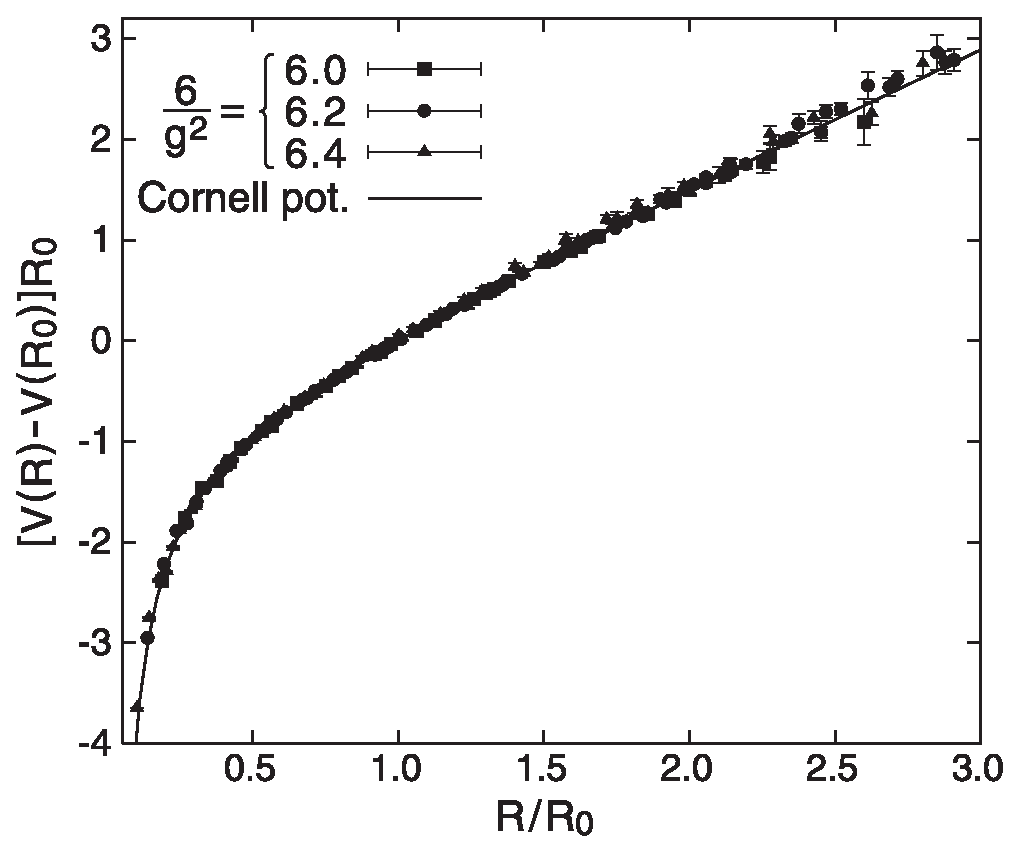
\includegraphics[scale=0.5]{Chapter3-figures/QQbar-pot.eps} 
 \end{center}
\caption{A dimensionless ${\rm Q}\bar{\rm Q}$ potential as a 
 function of a dimensionless quark$-$anti-quark
 separation $R/R_0$ with $R_0$ being the Sommer scale. 
 Different  symbols correspond to different lattice couplings
  $g(a)$    and hence different lattice spacings. 
  The solid line shows an empirical Cornell potential. 
  The figure is adapted from \cite{Bali:2000gf}.
  }
\label{fig:QQbar-pot}
\end{figure}
%%%%%%%%%%%%%%%%%%%%%%%%%%%%%%


%============================
\subsection{Masses of light hadrons}
%============================

 Meson masses and baryon masses can be 
 calculated with high accuracy by LQCD simulations
  with dynamical quarks.  The starting point is the hadronic 
  correlation functions $C_{\rm H=M,B} (n,n')$ in Eqs.(\ref{eq:correlation-M},\ref{eq:correlation-B}) 
  integrated over the spatial coordinates, $\vn$ and $\vn'$,   
 \beq
 \label{eq:5.D-tau}
 C_{\rm H}(\tau) = \sum_{\vn, \vn'} C_{\rm H} (n,n') 
 \xrightarrow[\tau \rightarrow \infty]
   \ |Z_{\rm H}|^2 {\rm e}^{-M_{\rm H} \tau}   ,
 \eeq   
where $\tau= (n_4-n_4')a$ is the temporal distance between the source at $n'$ and the sink at $n$,
 and  $M_{\rm H}$ ($Z_{\rm H}$) corresponds to the mass (the pole residue) 
 of a lightest bound state in each channel.
 If   the temporal extent of the 
  lattice is infinite, one can extract the 
   hadron mass from the formula,
  $M_{\rm H}= -(1/\tau) \ln C_{\rm H}(\tau)|_{\tau \rightarrow \infty} $.
  In practice, the {\it effective mass}  defined below is more useful,
 \beq
aM_{\rm H}^{\rm eff}(\tau) = \ln \left( \frac{C_{\rm H}(\tau)}{C_{\rm H}(\tau+a) } \right) .
\eeq
The asymptotic plateau of the effective mass at large $\tau$ corresponds to the hadron mass.
     In actual simulations,  the temporal extent is limited ($0 \le \tau/a \le \Ntau$), so that 
    the exponential damping 
    of  Eq.(\ref{eq:5.D-tau}) is replaced by
     $C_{\rm H} \rightarrow \exp[-M_{\rm H} \tau ] \pm  \exp [-M_{\rm H} (\Ntau a - \tau)]$
    where $+ (-)$ for the periodic (anti-periodic) boundary condition.
     
 Shown in the left panel of Fig.\ref{fig:hadron-mass} is the 
 dimensionless effective masses  ($a M_{\rm H}^{\rm eff}$)  against
 $\tau/a=(n_4-n_4')$ \cite{Durr:2008zz}.
  Data points are the effective masses for the pion $(\pi)$, the kaon $(K)$, the nucleon ($N$), the cascade baryon ($\Xi$) and 
  the omega baryon $(\Omega$)  calculated on the lattice with $a \simeq 0.085$ fm and 
  the pion mass $M_{\pi} \simeq 190$ MeV.  Reasonable plateau above $\tau/a > 9$ can
  be seen within the error bars.
 
 Shown in the right panel of Fig.\ref{fig:hadron-mass} is the 
 $M_{\pi}^2$-dependence of the $N$ and $\Omega$ masses for three different values of 
  $a$ \cite{Durr:2008zz}.
 The crosses are the values extrapolated to the continuum limit and to the physical pion mass.
 The $N$ and $\Omega$ masses predicted from LQCD and corresponding experimental numbers
 are 
\beq
\label{eq:mass-LQCD}
M_N^{\rm LQCD} &=& 0.936(25)(22)  \ {\rm GeV}, \ \ \ M_\Omega^{\rm LQCD} =1.676(20)(15)\ {\rm  GeV}, \\
M_N^{\rm exp.} &=& 0.939 \ {\rm  GeV}, \ \ \  \ \ \ \ \ \ \ \ \ \ \ \ \  M_\Omega^{\rm exp.} =1.672 \ {\rm  GeV}.
\eeq
  Note that the numbers in the first (second) parenthesis  in Eq.(\ref{eq:mass-LQCD}) 
 represent the statistical (systematic) errors on the last digits.

% FIG %%%%%%%%%%%%%%%%%%%%%%%%%%   
\begin{figure}[t]
\begin{center}
%\framebox[74mm]{\rule[-26mm]{0mm}{52mm}}
%\includegraphics[scale=0.6]{as-scale.eps}
\includegraphics[scale=0.29]{effective-mass.eps} \ \ 
\includegraphics[scale=0.28]{Chapter3-figures/NO_scaling.eps}
 \end{center}
\caption{(Left) The effective masses of hadrons against the 
 temporal separation between the source and the sink. 
(Right)  Hadron masses under the changes of the (pion mass)$^2$ as well as the lattice spacing $a$.
The figures are taken from \cite{Durr:2008zz}
  }
\label{fig:hadron-mass}
\end{figure}
%%%%%%%%%%%%%%%%%%%%%%%%%%%%%%%

Shown in Fig.\ref{fig:pn-mass} are the high precision numerical results of the 
 hadron mass splittings obtained by the 
 QCD+QED  lattice simulations with dynamical  $u,d,s,c$ quarks \cite{Borsanyi:2014jba}.
 The horizontal lines are the
experimental values and the grey shaded regions represent the experimental errors.
Red dots are the lattice results with their uncertainties denoted by the vertical error bars.
The neutron-proton mass differences from numerical simulations 
and the corresponding experimental numbers are
\beq
(M_n-M_p)^{\rm LQCD+QED} &=&\Delta N = 1.51(16)(23)\   {\rm MeV}, \\
(M_n-M_p)^{\rm exp.} &=& 1.29\   {\rm MeV}. 
\eeq

% FIG %%%%%%%%%%%%%%%%%%%%%%%%%%
\begin{figure}[t]
\begin{center}
%\framebox[74mm]{\rule[-26mm]{0mm}{52mm}}
%\includegraphics[scale=0.6]{as-scale.eps}
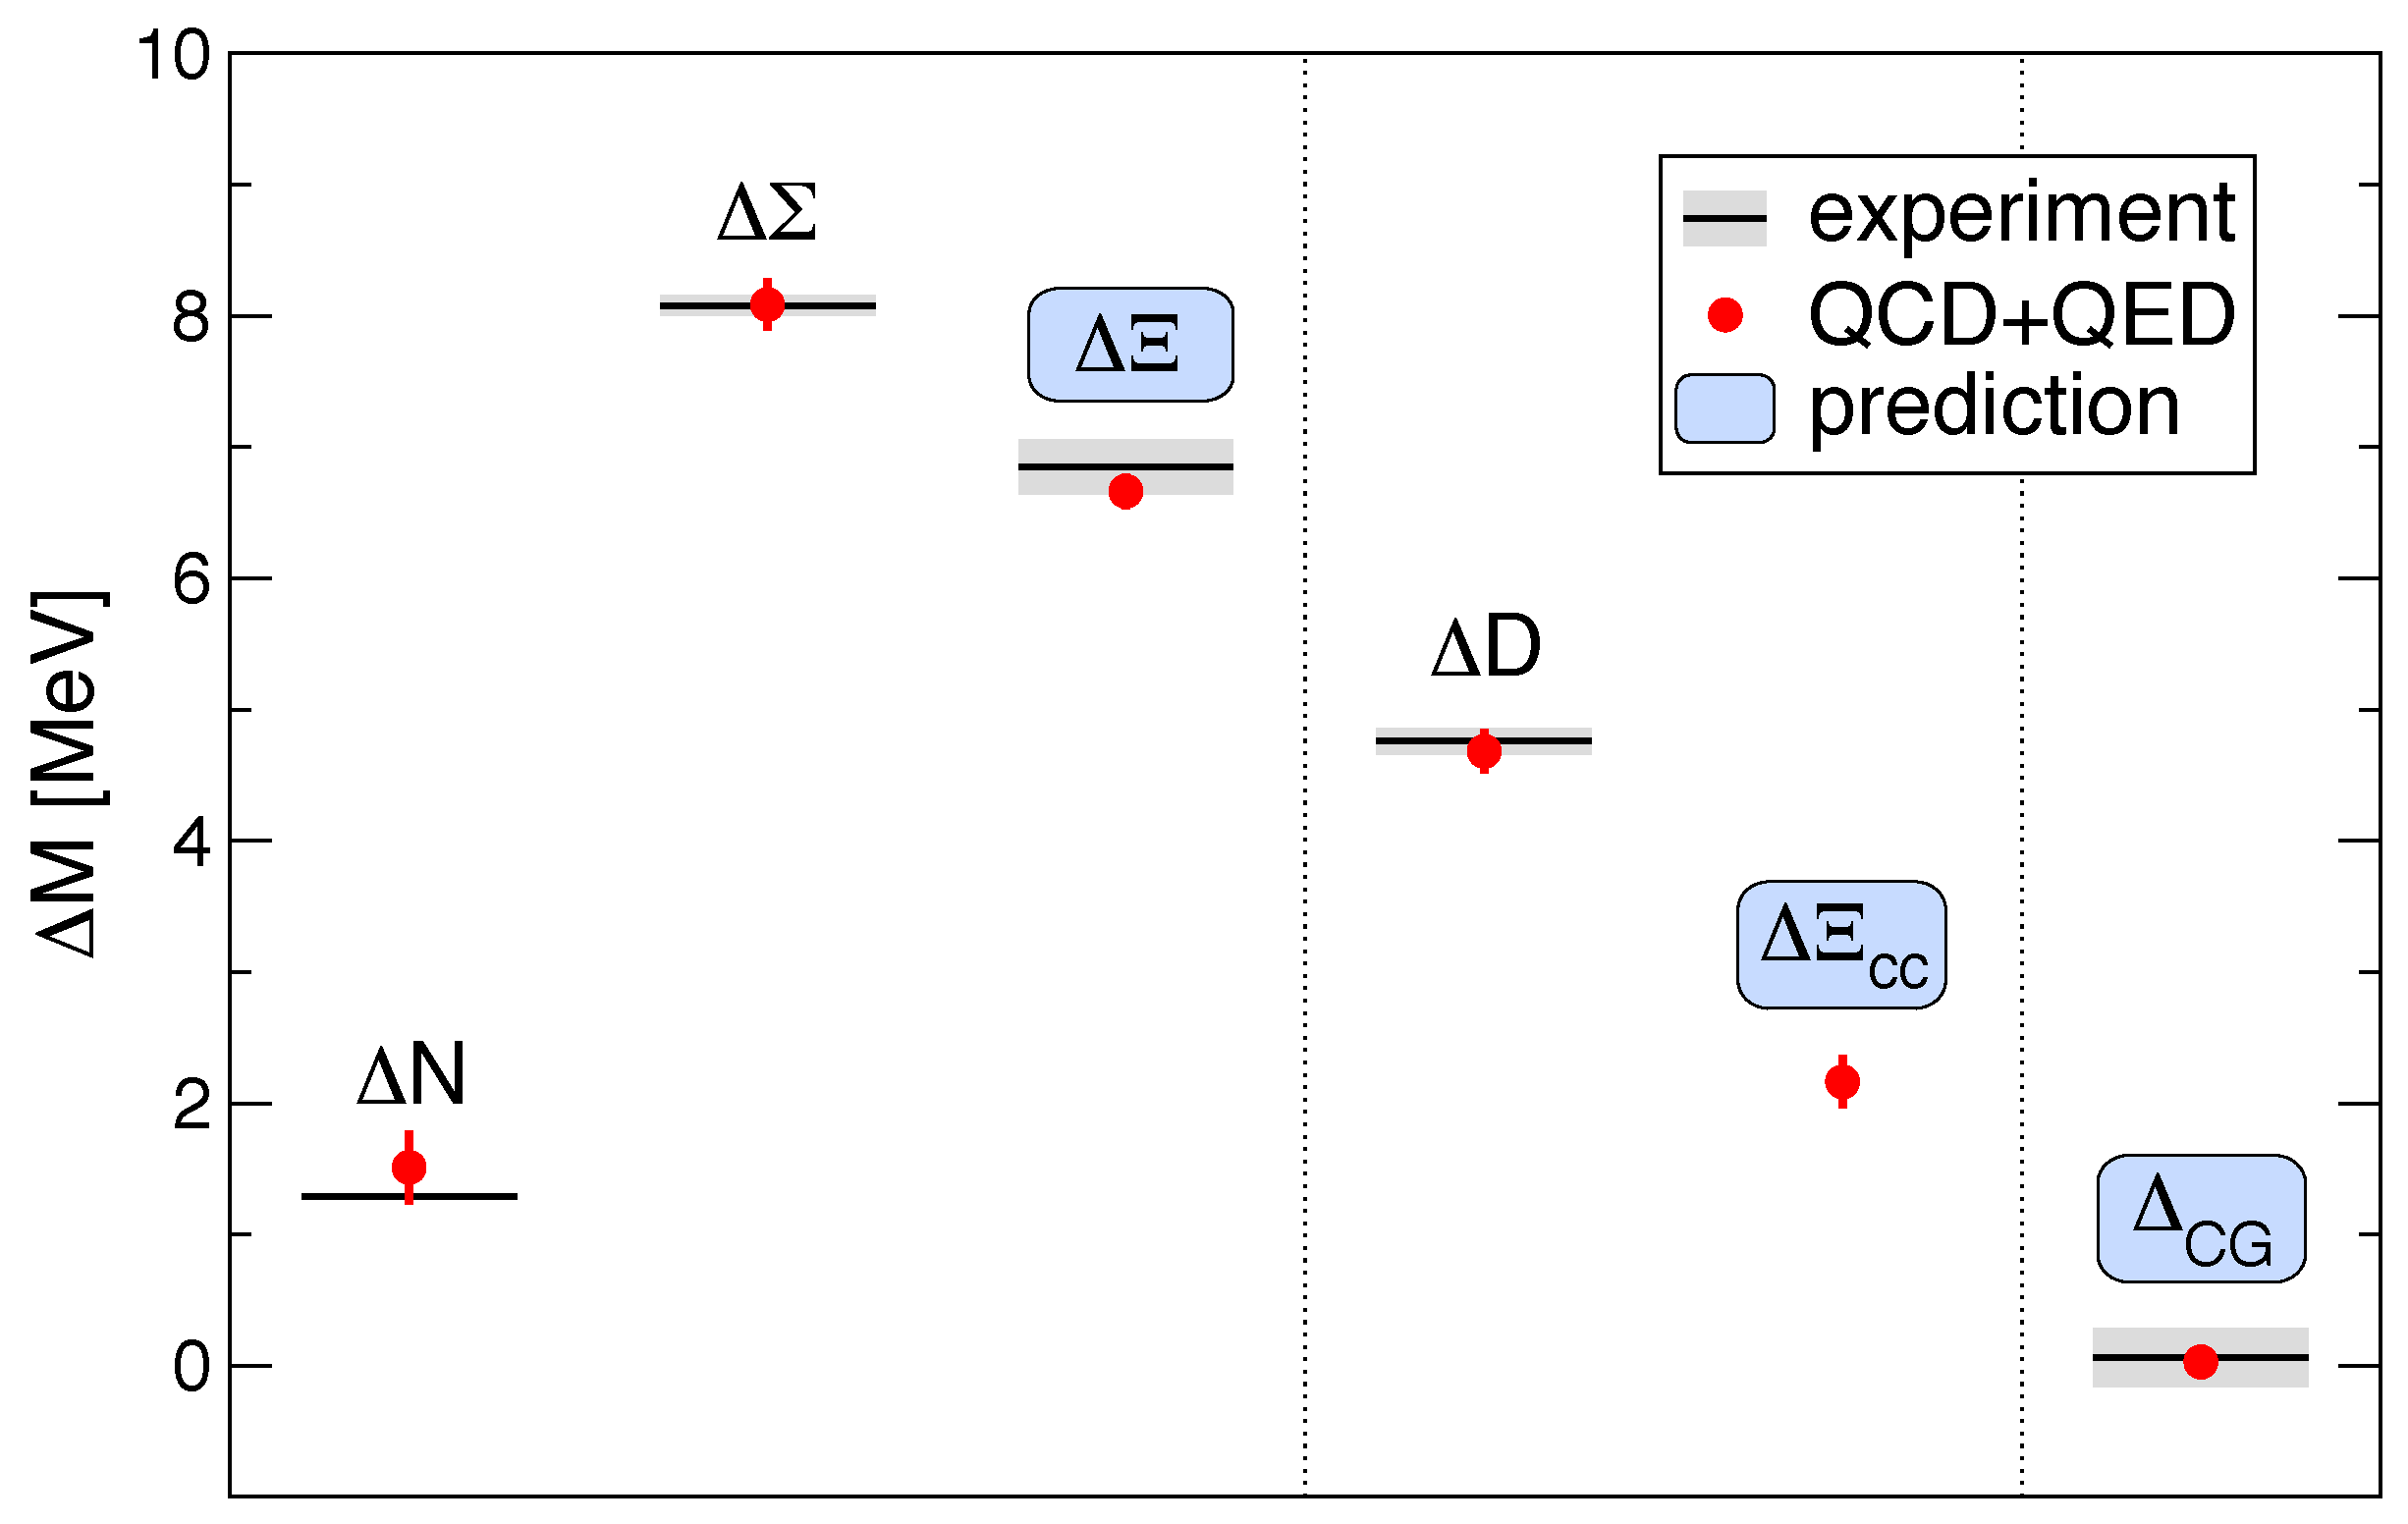
\includegraphics[scale=0.2]{Chapter3-figures/pn-mass.eps}
 \end{center}
\caption{Mass splittings in channels that are stable under the strong and electromagnetic interactions.
$\Delta N=M_n-M_p$, $\Delta \Sigma = M_{\Sigma^-}- M_{\Sigma^+}$,
$\Delta \Xi =M_{\Xi^-}- M_{\Xi^+}$,
$\Delta D= M_{D^{\pm}} - M_{D^0}$,
$\Delta \Xi_{cc} = \Delta \Xi_{cc}^{++} - \Delta \Xi_{cc}^{+}$,
$\Delta CG = \Delta N-\Delta \Sigma + \Delta \Xi$.
The figure is taken from
\cite{Borsanyi:2014jba}.
  }
\label{fig:pn-mass}
\end{figure}
%%%%%%%%%%%%%%%%%%%%%%%%%%%

Since all hadrons are composite particles of quarks and gluons,
there are numerous excited states  \cite{RPP}.  To extract the properties of the
excited hadrons from LQCD,  only looking at the asymptotic form as shown in Eq.(\ref{eq:5.D-tau}) is not
 sufficient, and more sophisticated methods such as  
 the maximal entropy method (MEM)  and  the variational method  are required.
 Interested readers should consult the reviews \cite{Asakawa:2000tr,Fodor:2012gf} and references there in.


%%%%%%%%%%%%%%%%%%%%%%%%
\section{Lattice QCD and nuclear force}
%%%%%%%%%%%%%%%%%%%%%%%%

Understanding of  the nuclear force from QCD
 is one of the most challenging problems in nuclear physics.
 Below the pion production threshold,
  the notion of the $NN$ potential (either in the coordinate space or in
  the  momentum space) has been known to be  useful, since it can be 
   used not only to describe the two-body system but also to 
   study  nuclear many-body problems through ab-initio calculations \cite{this_book}.
  Several high precision phenomenological $NN$ forces 
  have been constructed to reproduce
  the   neutron-proton and proton-proton scattering data (about 4500 data points)
   with a $\chi^2/{\rm dof} \sim 1$. However, 
     they have typically 20-40 fitting parameters:
   e.g. the CD Bonn potential, AV18 potential and N$^3$LO chiral effective field 
   theory have 38, 40, and 24 parameters, respectively \cite{Machleidt:2007ms}.
  If one tries to extend these to hyperon-nucleon and hyperon-hyperon interactions,
  the task becomes extremely tough since  the number of parameters 
   increases and the scattering data are scarce.
 
    Under this situation, it is highly desirable to
  study  baryon-baryon interactions from  first principle
  LQCD simulations, where  all the hadronic interactions are
   controlled only by the QCD coupling $g$  and 
    the quark mass $m$  whose values are
    pretty well determined at present by the precision QCD simulations \cite{Aoki:2013ldr}.
 
 The finite volume method (FVM), a
  theoretical framework to study hadron-hadron interactions
  from LQCD, was first  proposed 
  by L\"{u}scher \cite{luescher}: For two hadrons in a finite
  box with a spatial size $L^3$,  
  an exact relation between  the energy spectra in the box
  and the elastic scattering phase shift can be 
   derived.  If the range of the hadronic interaction $R_{\rm QCD}$  is sufficiently
  smaller than the size of the box $R_{\rm QCD}<L/2$, the behavior of the 
  the equal-time Bethe-Salpeter amplitude (or more precisely 
  the Nambu-Bethe-Salpeter (NBS) amplitude)
     $\psi (\vr)$ in the interval $R_{\rm QCD} < | \vr | < L/2 $
    has sufficient information to relate the phase shift and the 
  energy shift $\Delta E =M_{\rm HH}-2M_{\rm H}$.
  
   The HAL QCD method was proposed as another theoretical framework to study the hadron-hadron interactions from LQCD
 by Ishii, Aoki and Hatsuda \cite{Ishii:2006ec}
  and was further developed by  HAL QCD Collaboration \cite{HALQCD:2012aa}.
    The starting point is the same equal-time NBS amplitude  $\psi (\vr)$: 
  Instead of looking at the amplitude 
  outside the range of the interaction,
   the internal region $ |\vr | < R_{\rm QCD}$ is considered and
  an energy-independent  non-local potential $U(\vr, \vr')$  is deduced from  $\psi (\vr)$.
    Since $U(\vr, \vr')$ in QCD
   is spatially  localized due to the confinement
   of quarks and gluons, it is affected  only weakly
   by the finite lattice volume. Physical quantities such 
 as the scattering phase shifts, bound state spectra,  and resonance energies
  can be calculated by solving  the
  integro-differential differential equation satisfied by $\psi (\vr)$ with $U(\vr, \vr')$.
   
  Recently, a detailed comparison between the FVM and the HAL QCD method has been carried out:
  Although they agree with each other quite accurately for non-resonant pion-pion scattering,
   large signal to noise ratio  inherent in the effective mass $\Delta E^{\rm eff}(\tau)$  for 
    baryon-baryon scatterings prevents FVM to extract scattering observables   \cite{Iritani:2015dhu}.
   Therefore, we will focus on  the HAL QCD method below.
  
%=============================================     
\subsection{Master equation for baryon-baryon interaction}
%=============================================  
  
Let us consider  the baryon-baryon correlation in Fig.\ref{fig:correlation}(c) and 
define the equal-time NBS amplitude $\psi_{\ell}(\vr,\tau)$  from its large $\tau$ behavior:
 \beq
 C_{\rm BB}(\vr, \tau) 
 =\sum_{\vn',\vm'}   \left. C_{\rm BB}(n,m,n',m') \right|_{n_4=m_4,n_4'=m_4'} 
 \rightarrow \sum_{\ell} a_{\ell}  \psi_{\ell} (\vr,\tau)  e^{-E_{\ell} \tau}   ,
 \eeq 
 where $\vr=(\vn-\vm) a$, $\tau=(n_4-n_4')$, and $\psi_{\ell} (\vr,\tau)$ being the 
  NBS wave function for $\ell$-th scattering state on the lattice. 
  For large lattice size, $E_{\ell}$ is very dense, so that it is impossible to identify each level.  
 This causes a fatal problem in FVM as mentioned above.  On the other hand,
 if we define  $ C_{\rm BB}(\vr;\tau)= {\cal R}(\vr,\tau) e^{-2M_{\rm B} \tau}$, 
  the following  integro-differential equation can be derived below the inelastic threshold ($\tau > M_{\pi}^{-1}$),
\beq
  \left\{
  \frac1{4M_{\rm B}}\frac{\partial^2}{\partial \tau^2} 
  -\frac{\partial}{\partial \tau}
  - H_0
  \right\}
  {\cal R}(\vr,\tau)
  =
  \int d^3 r'
  U(\vr, \vr')
  {\cal R}(\vr', \tau),
  \label{eq.tdep}
\eeq
 with  $H_0= - \nabla^2/M_{\rm B}$.
 This is the master equation which has the 
correct information of the S-matrix and hence the scattering phase shift for
elastic $BB$ scatterings \cite{HALQCD:2012aa}.
  
  If we further focus on the 
  energies  much below  the inelastic threshold,
   the velocity expansion
   of $U(\vr,\vr')$ in terms of its  non-locality can be adopted.
   In fact, the potential with hermiticity, 
   rotational invariance, parity symmetry,   and time-reversal invariance may be expanded as \cite{okubo}
\begin{eqnarray} 
\label{eq:U-del}
  U(\vr,\vr')    &=& V(\vr, \vv) \delta(\vr-\vr'), \\
 V(\vr, \vv)    & =&
   \underbrace{V_{\rm C}(r) + V_{\rm T}(r) S_{12}}_{\rm LO} 
  + \underbrace{V_{\rm LS}(r) {\vL} \cdot {\vS}}_{\rm NLO}  
  +\underbrace{{O}(\vv^2)}_{{\rm N}^2{\rm LO}}
  + \cdots , 
   \label{eq:V-pot}
\end{eqnarray} 
   where $\vv = \vp/(M_{\rm B}/2) $, $\vL = \vr \times \vp $, 
   $\vp = -i \nabla$ and 
   $S_{12}=3(\vsigma_1 \cdot \vr)(\vsigma_2 \cdot \vr)/r^2 - \vsigma_1 \cdot \vsigma_2$.
     The central potential $V_{\rm C}$ and 
  the tensor potential $V_{\rm T}$ are classified as
  the leading order (LO) potentials since they
  are of $O(\vv^0)$. The next-to-leading (NLO) potential of  
  $O(\vv)$ is the spin-orbit potential  $V_{\rm LS}(r)$. 

%=============================================
\subsection{Baryon-baryon interaction in flavor SU(3) limit}
%=============================================  
  
 % FIG %%%%%%%%%%%%%%%%%%%%%%%%%%
\begin{figure}[t]
\begin{center}
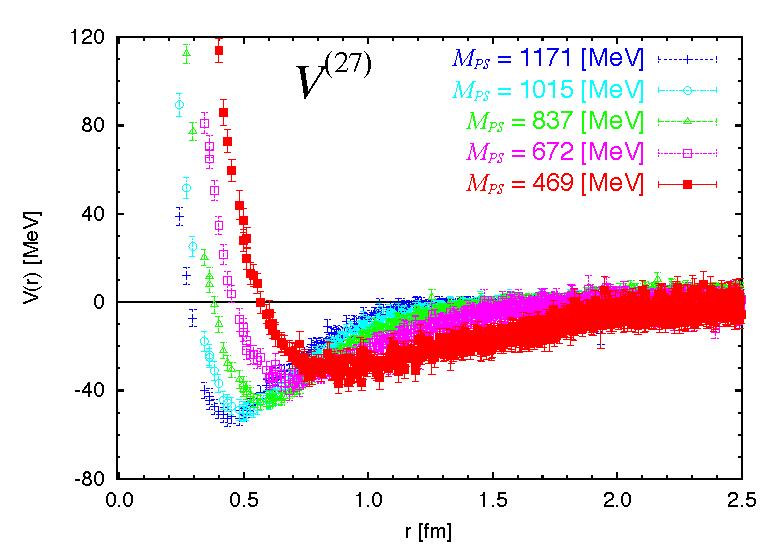
\includegraphics[scale=0.55]{Chapter3-figures/Vc_27_npa2.eps}\ \ \ \ \ \ \ 
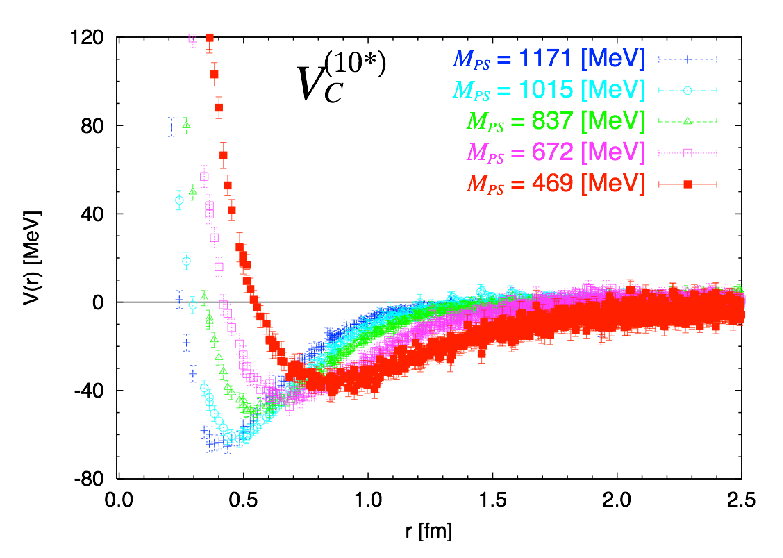
\includegraphics[scale=0.55]{Chapter3-figures/Vc_10s_npa2.eps}\\
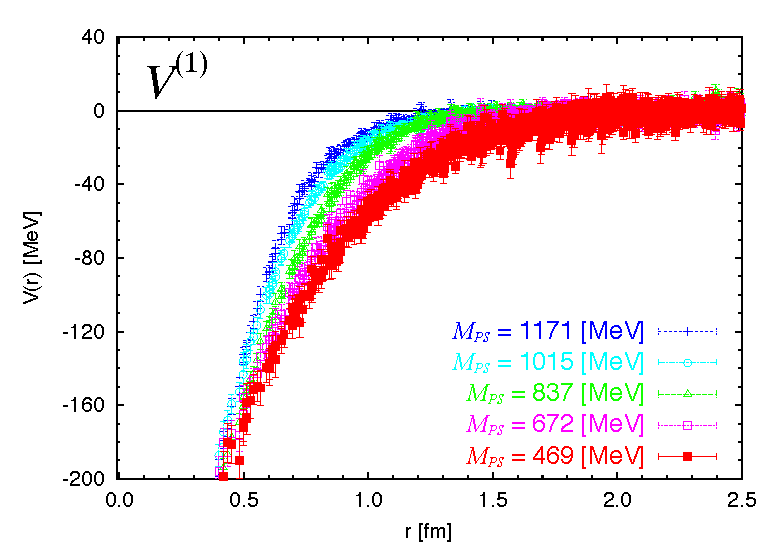
\includegraphics[scale=0.55]{Chapter3-figures/Vc_1_npa2.eps}\ \ \ \ \ \ \ 
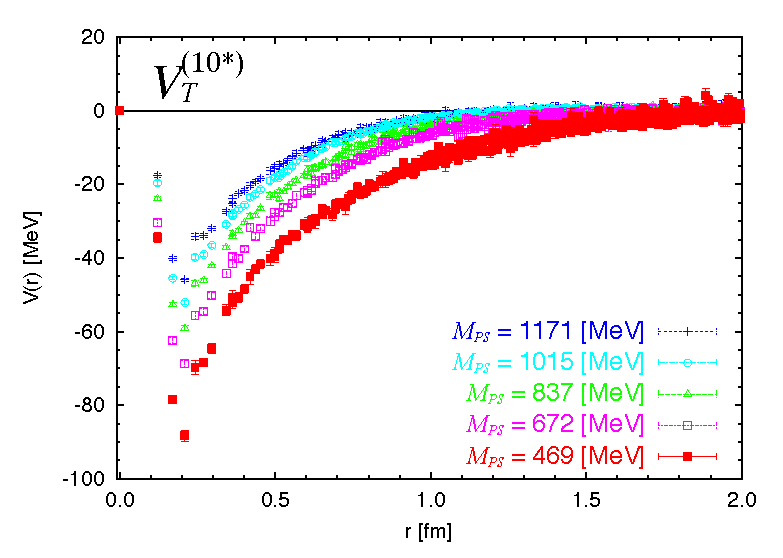
\includegraphics[scale=0.55]{Chapter3-figures/Vt_10s_npa2.eps}
 \end{center}
\caption{The baryon-baryon potentials from LQCD simulations in the flavour
SU(3) limit with several different masses of pseudo-scalar meson. 
The figures are taken from \cite{Inoue:2011ai}.
  }
\label{fig:NN-potential}
\end{figure}
%%%%%%%%%%%%%%%%%%%%%%%%%%%%%
  
 To obtain qualitative understandings of the nuclear force from QCD,
  the $S$-wave interaction between octet baryons  
 in the flavour SU(3) limit  would be a good starting point.
 In this case,  two baryon states with a given angular momentum
are labelled by the irreducible flavour multiplets,
\begin{equation}
 {\bf 8} \otimes {\bf 8} 
 = \underbrace{{\bf 27} \oplus {\bf 8}_s \oplus {\bf 1}}_{\mbox{symmetric}} ~ 
  \oplus \underbrace{{\bf 10}^* \oplus {\bf 10} \oplus {\bf 8}_a}_{\mbox{anti-symmetric}} \ . 
\end{equation}
Here ``symmetric" and ``anti-symmetric" stand for the symmetry under the
flavour exchange of two baryons.
For the system in the orbital S-wave, the Pauli principle between two baryons imposes 
${\bf 27}$, ${\bf 8}_s$ and ${\bf 1}$ to be spin singlet  ($^1S_0$) while 
${\bf 10}^*$, ${\bf 10}$ and ${\bf 8}_a$ to be spin triplet ($^3S_1$). 
Since there are no mixings among different multiplets in the SU(3) limit, 
one may define the corresponding potentials as
 \beq
^1S_0 \ &:& \  V^{({\bf 27})}(r), \ V^{({\bf 8}_s)}(r), \ V^{({\bf 1})}(r), 
\\ 
^3S_1 \ &:& \ V^{({\bf 10}^*)}(r), \ V^{({\bf 10})}(r), \ V^{({\bf 8}_a)}(r) ~.
\eeq
The diagonal potential ($B_1B_2 \rightarrow B_1 B_2)$ and  
 the off-diagonal potentials ($B_1B_2 \rightarrow B_3 B_4$) in the particle basis, 
 are obtained by  suitable combinations
of $V^{(\alpha)}(r)$ with $\alpha={\bf 27},{\bf 8}_s,{\bf 1},{\bf10}^*,{\bf 10},{\bf 8}_a$.

% FIG %%%%%%%%%%%%%%%%%%%%%%%%%%
\begin{figure}[t]
\begin{center}
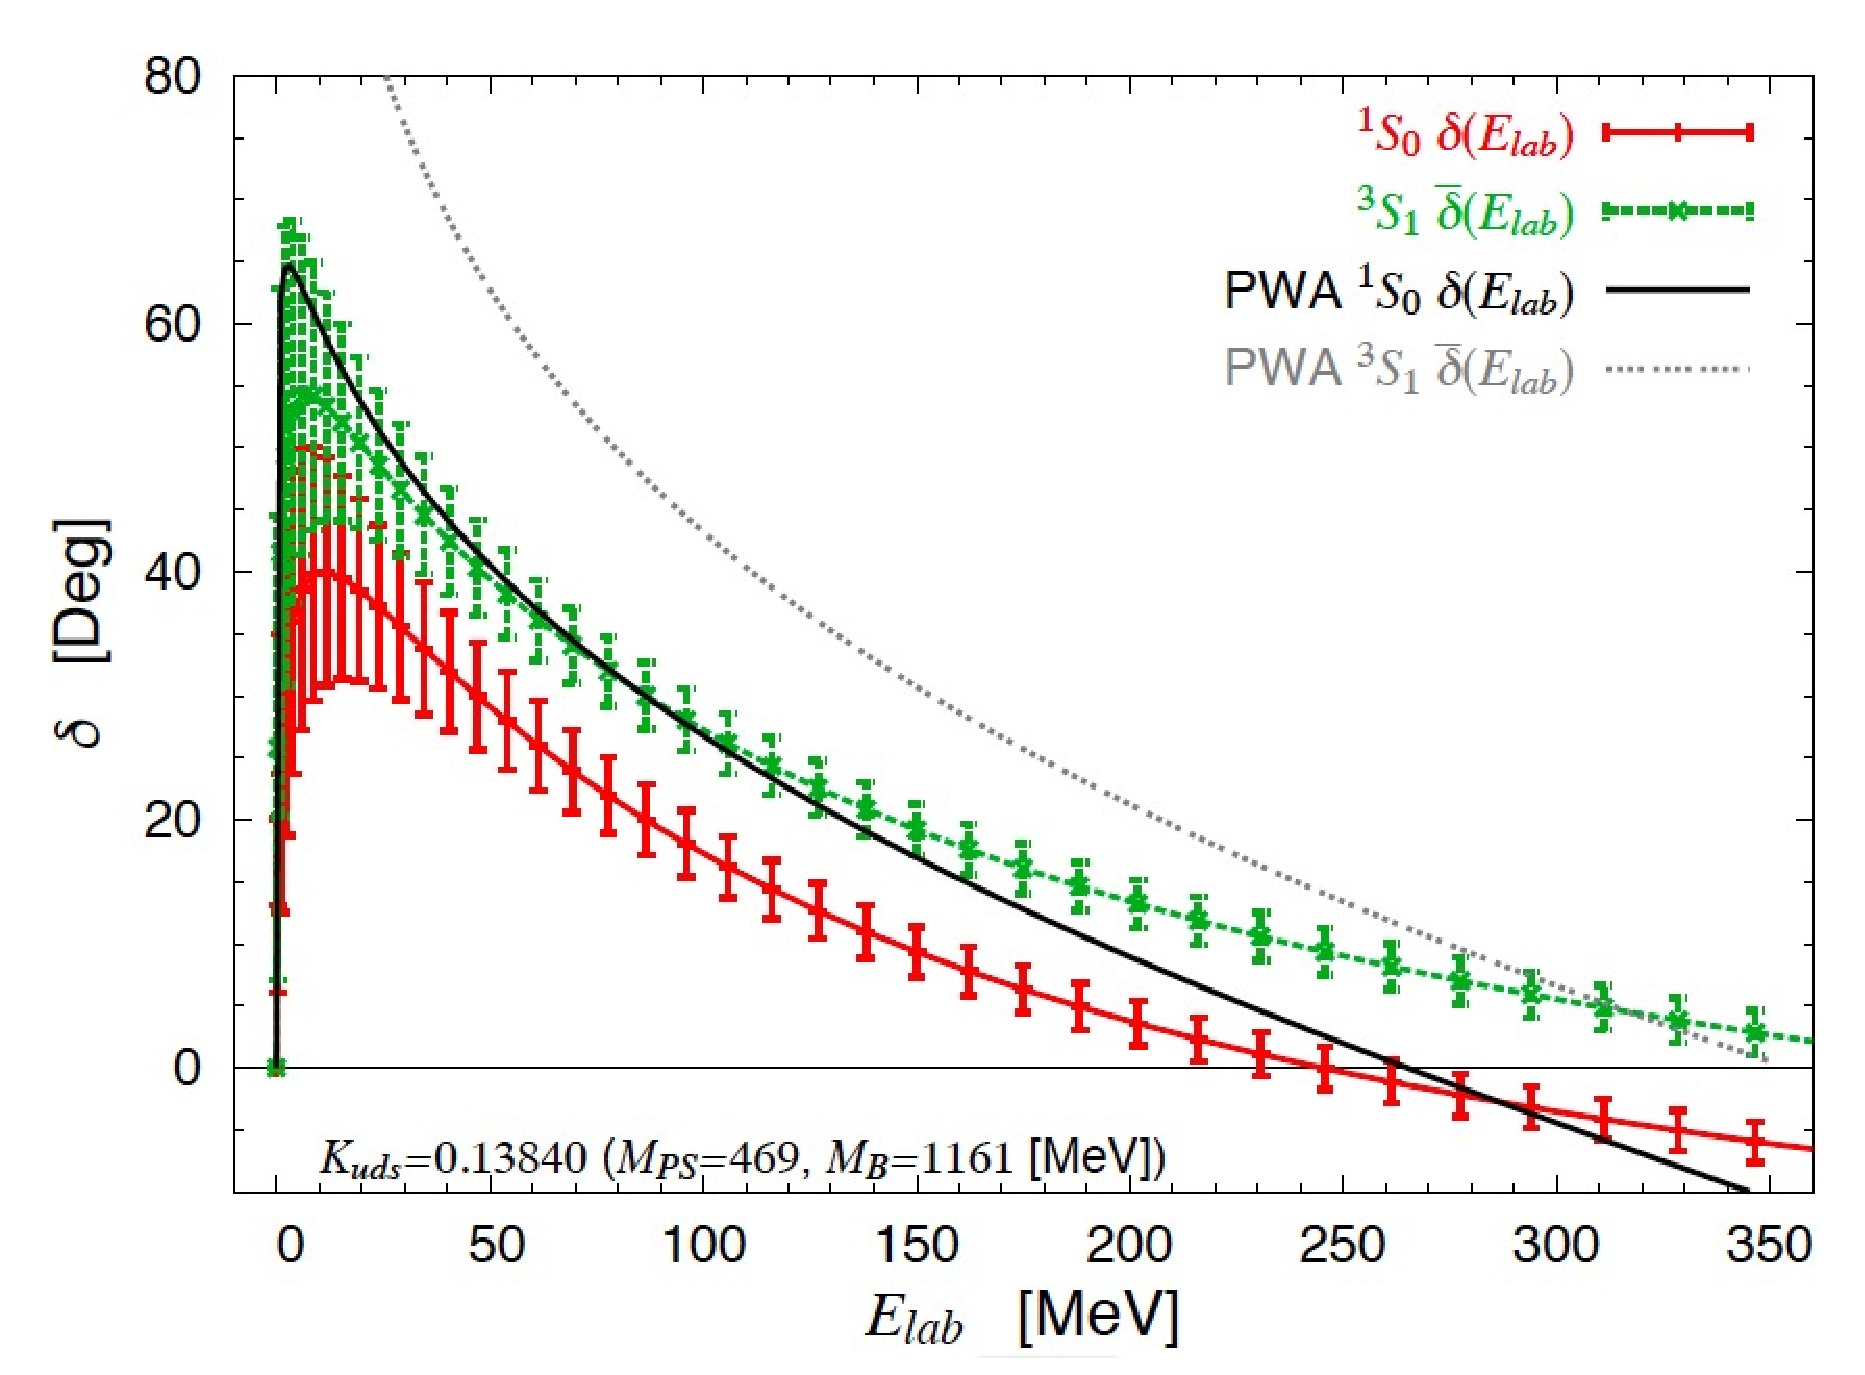
\includegraphics[scale=0.25]{Chapter3-figures/phase-shift.eps}\ \ \ \ 
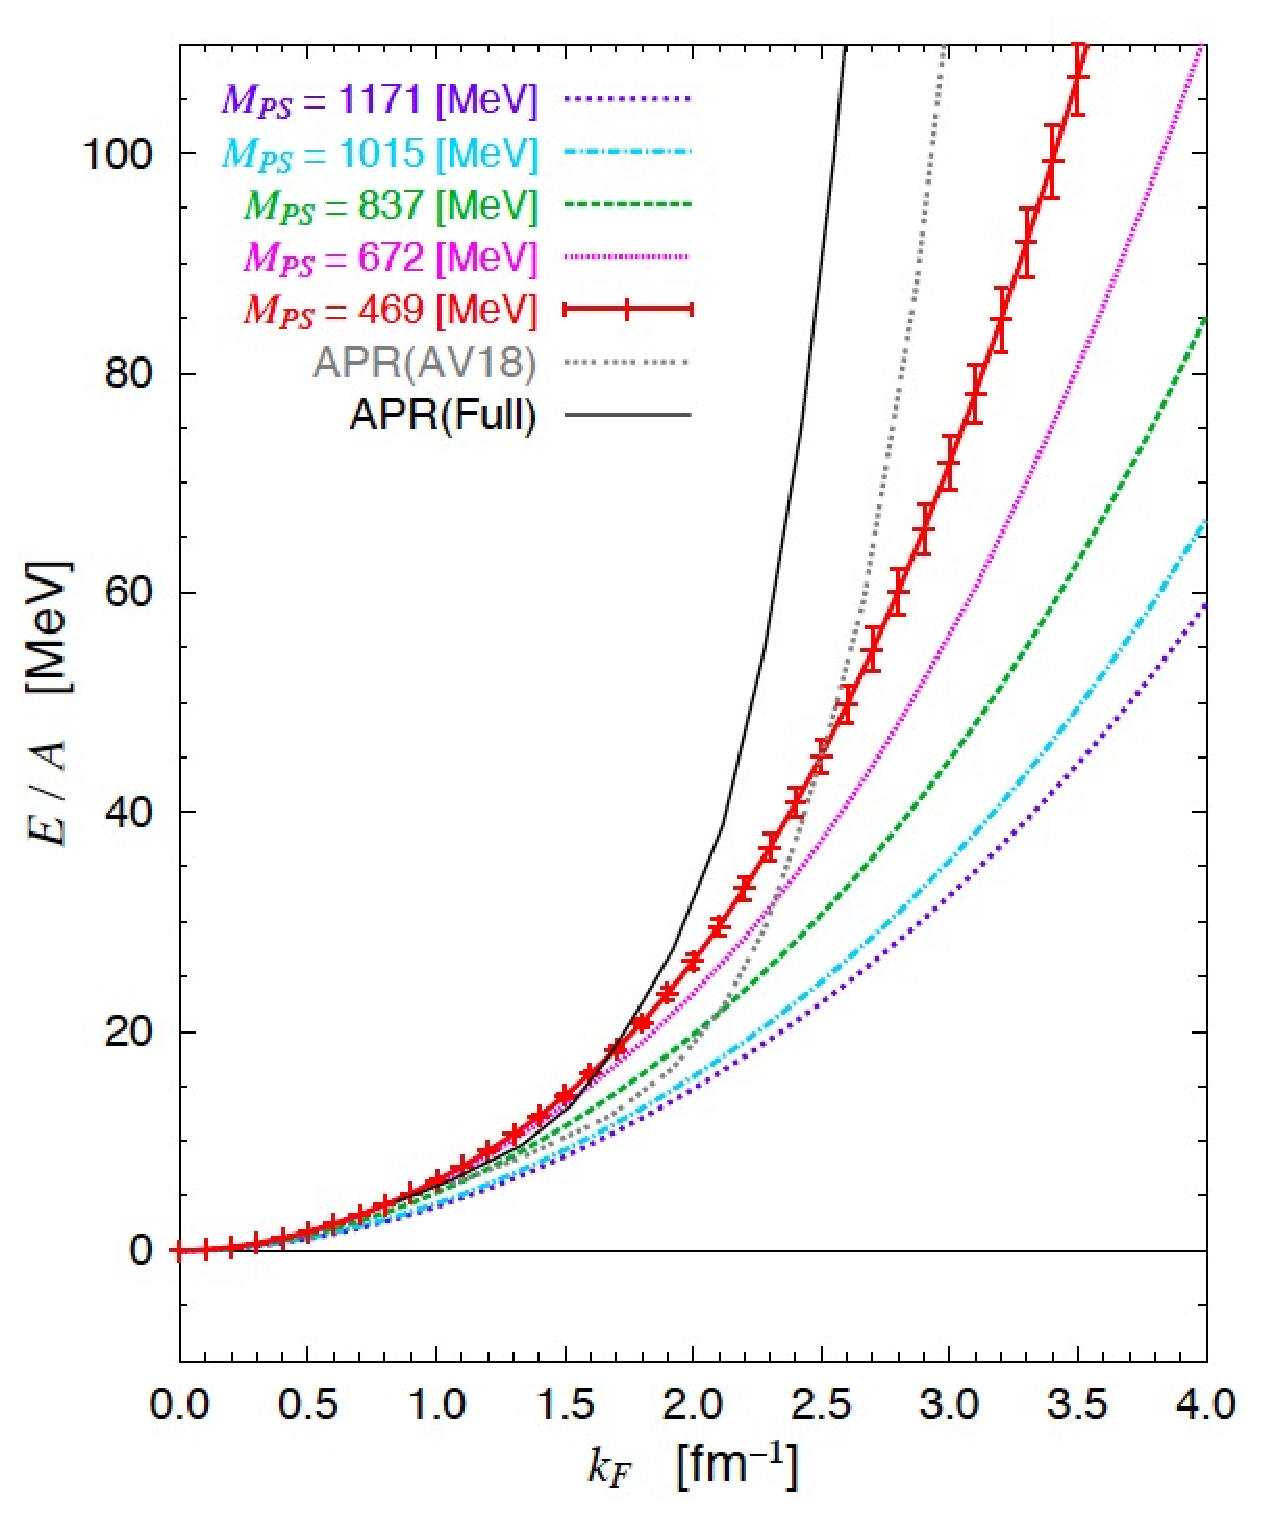
\includegraphics[scale=0.27]{Chapter3-figures/neutron-matter.eps}
 \end{center}
\caption{(Left) Phase shifts of the NN scattering as a
function of energy in the laboratory frame, extracted from
LQCD data at the pion mass 469 MeV in the flavor-SU(3) limit.
 The black and gray dashed lines are the results of the partial wave
analysis (PWA) of the experimental data. (Right) Ground state energy per neutron for the
pure neutron matter as a function of the Fermi momentum.
 The APR with black dotted line (black solid line)   corresponds to the empirical equation of state without (with) the
phenomenological three nucleon force \cite{Akmal:1998cf}.
 \cite{Akmal:1998cf}.
The figures are taken from \cite{Inoue:2013nfe}.
  }
\label{fig:NN-phase_shift}
\end{figure}
%%%%%%%%%%%%%%%%%%%%%%%%%%%%%%


Shown in Fig.\ref{fig:NN-potential}  are the results of the exploratory study of the potentials
obtained by LQCD simulations on the lattice  with $a\simeq 0.12$ fm, 
$L\simeq 4$ fm and 3 degenerate flavours  \cite{Inoue:2011ai}.  Corresponding pion mass ranges from
 469 MeV to 1171 MeV. 
\begin{itemize}
\item  The upper left panel is the 
central potential $V^{({\bf 27})}(r)$ to which the  $^1S_0$ nucleon-nucleon potential belongs.
 It  has a repulsive core at short distance and an attractive pocket at intermediate distance.
As the pion mass decreases,  the repulsive core gets stronger and the attractive tail gets
 longer.  
\item As shown in the lower left panel, the structure of the potential is quite different for $V^{({\bf 1})}(r)$ to which the
  flavour singlet $H$ dibaryon (composed of $uuddss$) belongs.   There is no repulsive core and the attraction 
  increases as the pion mass decreases.  Such a feature is consistent with the 
   notion of  the quark Pauli principle previous discussed in phenomenological quark models \cite{Oka-Fujiwara}.
\item The upper and lower right panels of  Fig.\ref{fig:NN-potential}  are the 
central potential and the tensor potential of $V^{({\bf 10}^*)}(r)$, respectively. The
$^3S_1$ nucleon-nucleon potential belongs to this channel. The central part has a similar
structure as the $^1S_0$ channel, while the tensor part has strong attraction and grows rapidly  as the 
 pin mass decreases.  The latter aspect is qualitatively consistent with the one-pion-exchange picture at
 long distances.
 \end{itemize}
   
 Shown in  Fig.\ref{fig:NN-phase_shift} (left) is  the nucleon-nucleon scattering phase shifts
  in the $^1S_0$ channel and $^3S_1$ channel obtained by using the 
   potentials, $V^{({\bf 27})}(r)$ and $V^{({\bf 10}^*)}(r)$,  for the pion mass 469 MeV \cite{Inoue:2013nfe}.
   The qualitative feature of the 
   phase shift in the $^1S_0$ channel is similar to the experimental one denoted by the 
   black solid  line, despite the fact that pion mass in the simulation is  more than 3 times
   heavier than the physical value. In the  $^3S_1$ channel, the deuteron bound state is 
   not formed yet due to heavy pion mass, so that the phase shift starts from 0 at zero energy
    in contrast the the experimental one denoted by the black dashed line.
    There is however a tendency that the attraction in the $^3S_1$ channel is larger than
   the $^1S_0$ channel even for the heavy pion mass.
  Shown in  Fig.\ref{fig:NN-phase_shift} (right) is  the energy per particle $E/A$ as a function of the 
  fermi momentum $k_{\rm F}$ for pure neutron matter calculated by using the Brueckner-Hartree-Fock method
  with the neutron-neutron potential in the $^1S_0$ channel in Fig.\ref{fig:NN-phase_shift} (left). 
 As the pion mass decreases, the equation of state becomes stiffer due to the growth of the repulsive  core. 
 The APR with black dotted line (black solid line)   corresponds to the empirical equation of state without (with) the
phenomenological three nucleon force  \cite{Akmal:1998cf}.

 We note that calculations of the baryon-baryon interactions  with  
  (2+1)-flavour LQCD on a large volume ($L \simeq 8.2 {\rm fm}$, $a\simeq 0.085$ fm) at
   nearly the physical quark mass ($m_{\pi}\simeq146$ MeV, $m_{K}\simeq$ 525 MeV)
   are underway  \cite{Doi:2015oha}.
 
  
%%%%%%%%%%%%%
\section{Exercises}
%%%%%%%%%%%%%

\begin{prob} \label{prob:1}
Prove the properties of the Wilson line, Eqs.(\ref{eq:5.wilson-line-i}), (\ref{eq:5.wilson-line-ii}), and (\ref{eq:5.wilson-line-iii}).
\end{prob}

\begin{prob}\label{prob:2}
Derive the expression on $U_{\mu \nu}(n)-1$ in 
Eq.(\ref{eq:5.wilson-plaq-cont-2}) by using the Baker-Campbell-Hausdorff formula.
\end{prob}

\begin{prob}\label{prob:3}
Show the $\Gamma_5$ Hermiticity of the Dirac operator in Eq.(\ref{eq:gamma5-hermite}).
\end{prob}

\begin{prob}\label{prob:4}
Derive  the free fermion propagator on the lattice in the momentum representation,
Eqs.(\ref{eq:DF}) and (\ref{eq:Mp}). 
\end{prob}

\begin{prob}\label{prob:5}
Analyze the dispersion relation of the free fermion associated with the 
Dirac operator, $D_{\rm GW}$ in Eq.(\ref{eq:5.overlap-op}).
\end{prob}

\begin{prob}\label{prob:6}
Derive the group integration formulas, Eq.(\ref{eq:group-int-1})- Eq.(\ref{eq:group-int-B}), by taking appropriate 
contractions of the color indices.
\end{prob}


\begin{prob}\label{prob:7}
Derive the formula for the Wilson loop in the strong coupling limit Eq.(\ref{eq:5.wilson-strong}) by using the group integration formulas
Eqs.(\ref{eq:group-int-0})-(\ref{eq:group-int-2}). 
\end{prob}

\begin{prob}\label{prob:8}
Derive the lattice coupling $g(a)$ as a function of the lattice spacing $a$, Eq.(\ref{eq:5.lat-running-g}).
\end{prob}

\begin{prob}\label{prob:9}
Show the convergence of $W[\phi]$ to the equilibrium distribution $W_{\rm eq}[\phi]$
under the Markov process by introducing the distance $D= \sum_{\phi} \left| W[\phi] -W_{\rm eq}[\phi] \right| $
 and by studying its behavior under update.
\end{prob}

\begin{prob}\label{prob:10}
Prove that the Metropolis test in Eq.(\ref{eq:MET-test})
satisfies the detailed balance Eq.(\ref{eq:DT-balance}).
\end{prob}

\begin{prob}\label{prob:11}
Derive the equation of motion for $P_l$ in Eq.(\ref{eq:EOM-P})
from Eq.(\ref{eq:EOM-U}) and  Eq.(\ref{eq:EOM-H}).
\end{prob}

\begin{prob}\label{prob:12}
Prove that the jackknife average and variance for $f({\cal O})={\cal O}$ reduce to the 
standard mean and unbiased variance, respectively.
\end{prob}

\begin{prob}\label{prob:13}
Prove that  the leapfrog integrator satisfies the reversibility Eq.(\ref{eq:reversible}) exactly.
Also prove that  the leapfrog integrator preserves the phase space area exactly by
evaluate the Jacobian, $d\phi' d\pi'= J d\phi d\pi $. 
\end{prob}
 

%%%%%%%%%%%%%%%%
\begin{acknowledgement}
%%%%%%%%%%%%%%%%
%If you want to include acknowledgments of assistance and the like at the end of an individual chapter 
%please use the \verb|acknowledgement| environment -- it will automatically render Springer's preferred layout.
The author thanks Takumi Doi and Atsushi Nakamura for useful comments and information on various aspects of
LQCD simulations.
He also thank the members of HAL QCD Collaboration for  fruitful discussions on the hadron-hadron interactions 
on the lattice.
This work was supported in part by MEXT SPIRE and JICFuS and also by RIKEN iTHES Project.
\end{acknowledgement}
%

\section{Appendix}
\addcontentsline{toc}{section}{Appendix}

%%%%%%%%%%%%%%%%%%%%%%%%%%%%
\subsubsection*{\center{Four vectors and Dirac matrices}}
%%%%%%%%%%%%%%%%%%%%%%%%%%%%

In the (3+1)-dimensional  Minkowski spacetime, coordinates, derivatives 
and four vectors with $\mu=0,1,2,3$ are
\beq
x^{\mu} = (t, \vx),
\ \ \partial^{\mu}   =  (\partial_t, -\nabla),
\ \  A^{\mu} =(A^0, \vA).
\label{eq:B.vector-M}
\eeq
In the 4-dimensional Euclidean space, 
 we define the corresponding vectors  for $\mu=4,1,2,3$ as
 \beq
(x_{\mu})^{\rm E} = (\tau=it, \vx),
\ \ (\partial_{\mu})^{\rm E}   =  (\partial_\tau = -i \partial_{t}, \nabla),
\ \  (A_{\mu})^{\rm E}  =(A_4=iA^0,\vA).
\label{eq:B.vector-E}
\eeq


In the (3+1)-dimensional  Minkowski spacetime with the 
 metric $g^{\mu \nu}={\rm diag}(1,-1,-1,-1)$,
  the Dirac matrices satisfy the following relations for $\mu=0,1,2,3$,
\beq
\{ \gamma^{\mu}, \gamma^{\nu} \} = 2 g^{\mu \nu},
\ \ \left( \gamma^{\mu} \right)^{\dagger} = \gamma^0 \gamma^{\mu} \gamma^0,
\ \ \gamma^5 &=& i \gamma^0 \gamma^1 \gamma^2 \gamma^3 
 = \gamma_5 = \left( \gamma_5 \right)^{\dagger}.
\label{eq:B.gamma-min}
\eeq
In the standard Dirac representation, we have
\beq
\gamma^0 = 
\left(  \begin{array}{cc}
        1   & 0   \\
        0   & -1  \\
        \end{array}  \right) , \ \ 
\gamma^j = 
\left(  \begin{array}{cc}
        0           & \sigma_j   \\
        -\sigma_j   & 0          \\
        \end{array}  \right) , \ \ 
\gamma^5 =
\left(  \begin{array}{cc}
        0   & 1   \\
        1   & 0   \\
        \end{array}  \right)  ,
\eeq
where $\sigma_j$ are the Pauli matrices;        
$
%\beq
\sigma_1 = 
\left(  \begin{array}{cc}
        0   & 1   \\
        1   & 0   \\
        \end{array}  \right) , 
\sigma_2 = 
\left(  \begin{array}{cc}
        0           & -i   \\
        i           & 0    \\
        \end{array}  \right) , 
\sigma_3 =
\left(  \begin{array}{cc}
        1   & 0    \\
        0   & -1   \\
        \end{array}  \right)  .
%\label{eq:B.Pauli-matrix}
%\eeq
$

In the 4-dimensional Euclidean space  with the metric
 $\delta_{\mu \nu}={\rm diag}(1,1,1,1)$, we define
  the Euclidean Dirac matrices as
 \beq
  \Gamma_{\mu}  \equiv
 \left(\gamma_4= \gamma^0, -i \vgamma \right),  
 \ \ \Gamma_{-\mu} \equiv  - \Gamma_{\mu}, 
  \ \ {\rm and}   \ \ \Gamma_5 \equiv \gamma^5,
  \eeq
 which satisfy the relations,
 \beq
 \{ \Gamma_{\mu}, \Gamma_{\nu} \}  = 2 \delta_{\mu \nu},
\ \ \Gamma_{\mu}^{\dagger} = \Gamma_{\mu} , 
\ \ \ \ ({\rm for} \ \mu=1,2,3,4,5) 
\label{eq:B.gamma-lat} 
\eeq 

%%%%%%%%%%%%%%%%%%%%%
\subsubsection*{\center{SU$(N)$ algebra}}
%%%%%%%%%%%%%%%%%%%%%

Let ${\cal T}^a$ ($a=1, \cdots , N^2-1$) are the 
 Hermitian generators of the SU$(N)$ group. They satisfy
  the Lie algebra  \index{Lie algebra}
\beq
\left[  {\cal T}^a , {\cal T}^b \right] = i f_{abc} {\cal T}^c ,
\eeq
where $f_{abc}$ is the structure constant \index{structure constants}
 being totally anti-symmetric in its indices.
 $({\cal T}^b)^2$ commutes with every generator ${\cal T}^a$
  and   is called the quadratic Casimir operator. 
  
 For $N=2$, $f_{abc}$ reduces to the  anti-symmetric
 tensor $\epsilon_{ijk}$ with  $\epsilon_{123}=1$.
For $N=3$, the non-vanishing components of $f_{abc}$ read
$f_{123}=1, f_{147}=-f_{156}=f_{246}=f_{257}=f_{345}=-f_{367}=1/2,  
f_{458}=f_{678}= {\sqrt{3}}/{2}$.
   
  In the fundamental representation, 
 ${\cal T}^a$ is written by the $N \times N$ matrices $t^a$ as
\beq
t^a = \frac{1}{2} \lambda_a,
\eeq
 where $\lambda_a$ for $N=2$ reduce to  the Pauli matrices 
 $\sigma_i$, while  those for $N=3$ reduce to the Gell-Mann matrices.
 
 Some useful relations of $t^a$ for general $N$ are
\beq
\label{eq:tt}
{\rm tr} (t^a t^b) = \frac{1}{2} \delta_{ab}, 
\ \ \ t_{ij}^a t_{kl}^b  =  \frac{1}{2} (\delta_{il}\delta_{jk} -\frac{1}{N} \delta_{ij}\delta_{kl} ),
\ \ \ (t^a t^a)_{ij} = C_{{\rm F}} \delta_{ij},
\ \ \ {\rm with} \ C_{{\rm F}}=\frac{N^2-1}{2N}.
\eeq
   
In the adjoint representation, \index{adjoint representation}
 ${\cal T}^a$ is written by  $(N^2-1) \times (N^2-1)$ matrices $T^a$ as
\beq
(T^a)_{bc} = -i f_{abc} ,
\eeq
which satisfy the relations
\beq
  {\rm tr} (T^a T^b) &=& N \delta_{ab}, 
  \ \ \  (T^a T^a)_{bc} = C_{{\rm A}} \delta_{bc},
  \ \ \  {\rm with} \ C_{{\rm A}}= N.
\eeq



%%%%%%%%%%%%%%%%%%%%%%%%%%%%%%
\subsubsection*{\center{Gaussian and Grassmann integrals}}
%%%%%%%%%%%%%%%%%%%%%%%%%%%%%%
 
Basic Gaussian and Grassmann integrals are 
\beq
 \label{eq:C.gauss-x}
& &\int_{-\infty}^{+\infty} \frac{dx}{\sqrt{2\pi}}\ {\rm e}^{-ax^2/2} 
    =\frac{1}{\sqrt{a}}, \\
 \label{eq:C.gauss-z}
& & \int \frac{dz^* dz}{2 \pi i}\ {\rm e}^{-b |z|^2} = \frac{1}{b}, \\
 \label{eq:C.gauss-xi}
& & \int d\bar{\xi} d\xi\  {\rm e}^{- c \bar{\xi} \xi} = c .
\eeq     
Here $x$ ($z$) is a real (complex) number, while $\bar{\xi}$ and
 $\xi$ are anti-commuting Grassmann numbers ($\{ \xi, \bar{\xi} \} =0$,
 and  $\xi^2 = \bar{\xi}^2=0$).
 $a$ and $b$ are assumed to be real and positive numbers, while $c$ is an
  arbitrary complex number.
 Eq.(\ref{eq:C.gauss-z}) can be shown by rewriting the integral 
 in terms of the real and imaginary parts of $z$ or in terms of the 
 polar coordinates of $z$.   Eq.(\ref{eq:C.gauss-xi})
  can be shown by noting that 
   ${\rm e}^{-c\bar{\xi}\xi} = 1- c \bar{\xi}{\xi}$
   and $ \int d\xi = \partial/\partial \xi $
   (integral = derivative) for Grassmann variables.
  
Generalization of the above results to the case of multiple variables
 is straightforward.  For $x =(x_1, \cdots, x_n)$, 
  $z =(z_1, \cdots, z_n)$, $\xi =(\xi_1, \cdots, \xi_n)$,
 and $\bar{\xi} =(\bar{\xi}_1, \cdots, \bar{\xi}_n)$ with
  $\{ \xi_k, \xi_l \} = \{ \bar{\xi}_k, \bar{\xi}_l \} 
   = \{ \xi_k, \bar{\xi}_l \} =0$,  we have
 \beq
 \label{eq:C.gauss-xn}
& &\int \prod_{l=1}^n \frac{dx_l}{ \sqrt{2\pi} }\ 
 {\rm e}^{-\frac{1}{2} x A x} = \frac{1}{\sqrt{{\rm Det}\ A}}, \\
 \label{eq:C.gauss-zn}
& & \int \prod_{l=1}^n \frac{dz_l^* dz_l}{2 \pi i}\ 
{\rm e}^{- z^* B z} = \frac{1}{{\rm Det}\ B}, \\
 \label{eq:C.Z-grass-xin}
& & \int \prod_{l=1}^n d\bar{\xi}_l d\xi_l \
  {\rm e}^{- \bar{\xi}C \xi} = {\rm Det}\ C .
\eeq  
Here $A$ is a non-singular and real-symmetric matrix whose
 eigenvalues $a_l$ satisfy $a_l > 0$ for all $l$.
 $B$ is a non-singular complex matrix whose complex eigenvalues $b_l$
  obtained by the 
  biunitary transformation ($U B V^{\dagger}$)  
  satisfy ${\rm Re}\ b_l > 0$ for all $l$.
 $C$ is an arbitrary complex matrix with no conditions. 
 Note that $B$ and $C$ do not have to be Hermitian matrices.
 In field theories, the label ``$l$" summarizes all possible indices including
  spin, flavor, color, spacetime points etc. and 
  ``${\rm Det}$" denotes the determinant for all these indices. 
 


%%%%%%%%%%%%%%%%%%%%%%%%%%
\subsubsection*{\center{Method of characteristics}}
%%%%%%%%%%%%%%%%%%%%%%%%%%

We need to construct  a general  solution of the 
following partial differential equation,
\beq
 \left( \lambda \frac{\partial}{\partial \lambda} + \beta(g) \frac{\partial}{\partial g} \right) f(\lambda,g)=0.
 \label{eq:MCA-1}
 \eeq
 For this purpose, we introduce the running coupling $\bar{g}(\lambda)$ through 
 $\lambda d\bar{g}/d\lambda = -\beta(\bar{g})$ whose formal solution reads
 \beq
 \lambda = \exp \left( - \int_g^{\bar{g}(\lambda) }  \frac{dg'}{\beta(g')}  \right) .
 \label{eq:MCA-2}
  \eeq
 Then the solution of Eq.(\ref{eq:MCA-1}) can be written as 
 \beq
 f(\lambda, g) = f (1, \bar{g} (\lambda)).
 \eeq
 This can be explicitly checked  by applying the partial derivative on both sides,
 \beq
  \lambda \partial_{\lambda}  f(\lambda,g)&=&
  \lambda (\partial_{\lambda} \bar{g})   (\partial_{\bar{g}} f) = - \beta (\bar{g})  (\partial_{\bar{g}} f) , \nonumber \\
  \beta \partial_g f(\lambda,g) &=&
  \beta(g) \left. (\partial \bar{g}/\partial g) \right|_{\lambda}  (\partial_{\bar{g}} f) = \beta (\bar{g})  (\partial_{\bar{g}} f) .
 \eeq 
 where we have used the  relation $\partial \bar{g}/\partial g = \beta(\bar{g})/\beta(g)$ 
  obtained from   Eq.(\ref{eq:MCA-2}).
 
 In general, the first-order partial differential equation (PDE)  can be transformed to 
 a set of ordinary   differential equations (ODEs) and can  be solved by  {\it the method of characteristics}. 
 As an illustration,  let us consider the following PDE, 
 \beq
  a(t,x) \partial_t u(t,x) + b(t,x) \partial_x f(t,x) = c(t,x).
\label{eq:MCA-3}
 \eeq
This is equivalent to the coupled ODEs,
\beq
\frac{d \bar{t}}{ds}  = a (\bar{t}, \bar{x}) , \ \ 
\frac{d \bar{x}}{ds}  = b (\bar{t}, \bar{x}) , \ \ 
\frac{d f(\bar{t},\bar{x} ) } {ds}  = a (\bar{t}, \bar{x}) ,
\label{eq:MCA-4}
\eeq
where $s$ parametrizes the  "flow" of the coordinates. $(\bar{t}(s), \bar{x}(s))$.
This is called the {\it characteristic curve} as shown in Fig.\ref{fig:char-c}.

\begin{figure}[t]
\begin{center}
%\framebox[74mm]{\rule[-26mm]{0mm}{52mm}}
%\includegraphics[scale=0.6]{as-scale.eps}
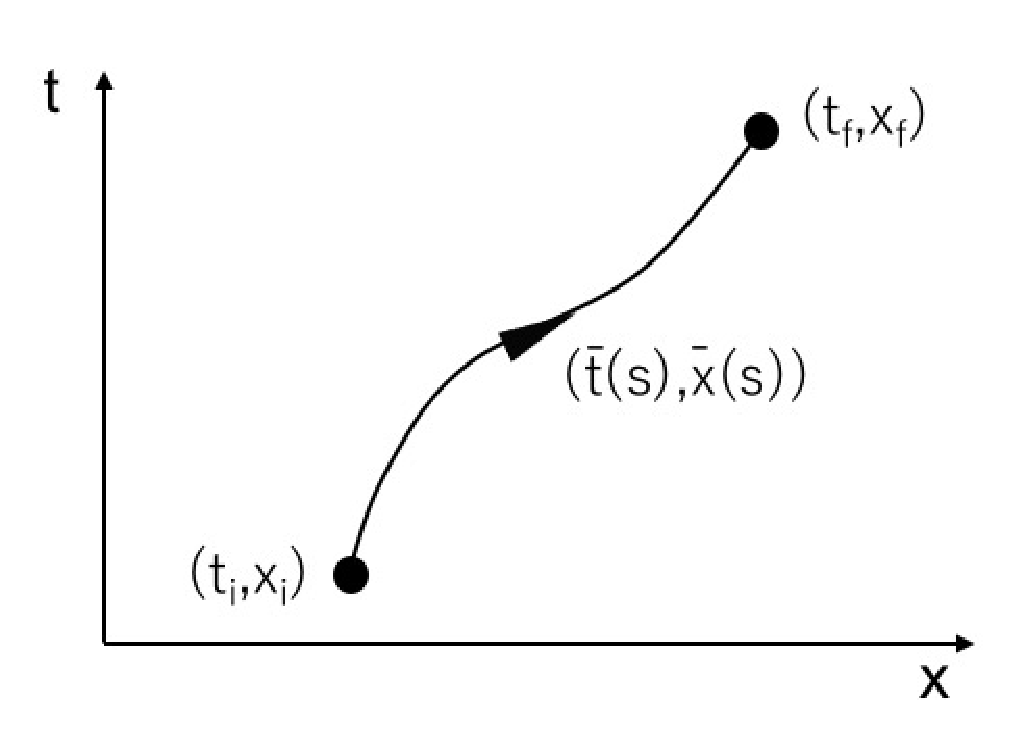
\includegraphics[scale=0.35]{Chapter3-figures/char-c.eps} 
 \end{center}
\caption{Schematic illustration of the characteristic curve.}
\label{fig:char-c}
\end{figure}

The function $f$ can be obtained by integrating the last equation of Eq.(\ref{eq:MCA-4}) 
on the  characteristic curve from the initial point $(t_{\rm i},x_{\rm i})$ to the final point $(t_{\rm f},x_{\rm f})\equiv (t,x)$,
\beq
f(t,x)= f (t_{\rm i}, x_{\rm i}) + h (t, x, t_{\rm i}, x_{\rm i})
\label{eq:MCA-6}
\eeq
where  $h$ stands for an integration of the known function $c(\bar{t},\bar{x})$ on the
characteristic curve.  Eq.(\ref{eq:MCA-6}) implies  that the desired function at $(t,x)$ is obtained 
essential by a "pullback" of the point to $(t_{\rm i},x_{\rm i})$ along the characteristic curve. 
It is a straightforward exercise  to generalize the above derivation to the system with more coordinates,
$(t, \vx)$.  

%%%%%%%%%%%%%%%%%%%%%%%%%%%%%%%%%%
 \subsubsection*{\center{Leapfrog integrator in molecular dynamics}}
%%%%%%%%%%%%%%%%%%%%%%%%%%%%%%%%%%

Let us start with a Tayler expansion of the field $\phi$:
\beq
\label{eq:LF-phi}
\phi(s+\varepsilon) &=& \phi(s) + \varepsilon \dot{\phi}(s) + \frac{\varepsilon^2}{2} \ddot{\phi}(s) + O(\varepsilon^3), \nonumber \\
&=&  \phi(s) + \varepsilon {\pi}(s) + \frac{\varepsilon^2}{2} \dot{\pi}(s) + O(\varepsilon^3), \nonumber  \\
&=& \phi(s) + \varepsilon {\pi}(s+\varepsilon/2) + O(\varepsilon^3), 
\eeq
where we have used the equation of motion, $\dot{\phi}(s) \equiv d\phi(s)/ds = \pi(s)$.
To evaluate ${\pi}(s+\varepsilon/2)$, we take the midpoint prescription which does not have $O(\varepsilon^2)$ error,
 \beq
 \label{eq:LF-pi}
{\pi}(s+\varepsilon/2)&=&{\pi}(s-\varepsilon/2) + \varepsilon \dot{\pi}(s) + O(\varepsilon^3) \nonumber \\
&=&  {\pi}(s-\varepsilon/2)   - \varepsilon \frac{\delta S(\phi)}{\delta \phi(s)} + O(\varepsilon^3) .
\eeq
Eqs.(\ref{eq:LF-phi}) and (\ref{eq:LF-pi})  give a procedure to move the molecular dynamics one-step forward,
$(\phi(s), \pi(s-\varepsilon/2))  \rightarrow (\phi(s+\varepsilon), \pi(s+\varepsilon/2))$. 
The initial and final steps need to receive special care,
\beq
\pi(\varepsilon/2) = \pi(0) - \frac{1}{2} \varepsilon \frac{\delta S(\phi)}{\delta \phi(s)} + O(\varepsilon^2), \ \ \ 
\pi(s_{\rm f}) =\pi(s_{\rm f}-\varepsilon/2) -  \frac{1}{2} \varepsilon \frac{\delta S(\phi)}{\delta \phi(s_{\rm f})} + 
O(\varepsilon^2),
 \eeq
 which have only $O(\epsilon^2)$ accuracy.  An illustration of this leapfrog integrator is shown in Fig.(\ref{fig:LF}).
 Since the initial and final steps introduce  $O(\varepsilon^2)$ error irrespective of the 
length of the MD trajectory, and  the intermediate steps introduce 
$O(\varepsilon^3) \times \varepsilon^{-1} =O(\varepsilon^2)$ error as a whole,  one finds
 $\Delta H = O(\varepsilon^2)$ after one MD trajectory before the Metropolis test.

The leapfrog integrator satisfies the reversibility and symplectic property, which can be checked explicitly
by using the above definitions (Exercise \ref{prob:13}).
 
 \begin{figure}[t]
\begin{center}
%\framebox[74mm]{\rule[-26mm]{0mm}{52mm}}
%\includegraphics[scale=0.6]{as-scale.eps}
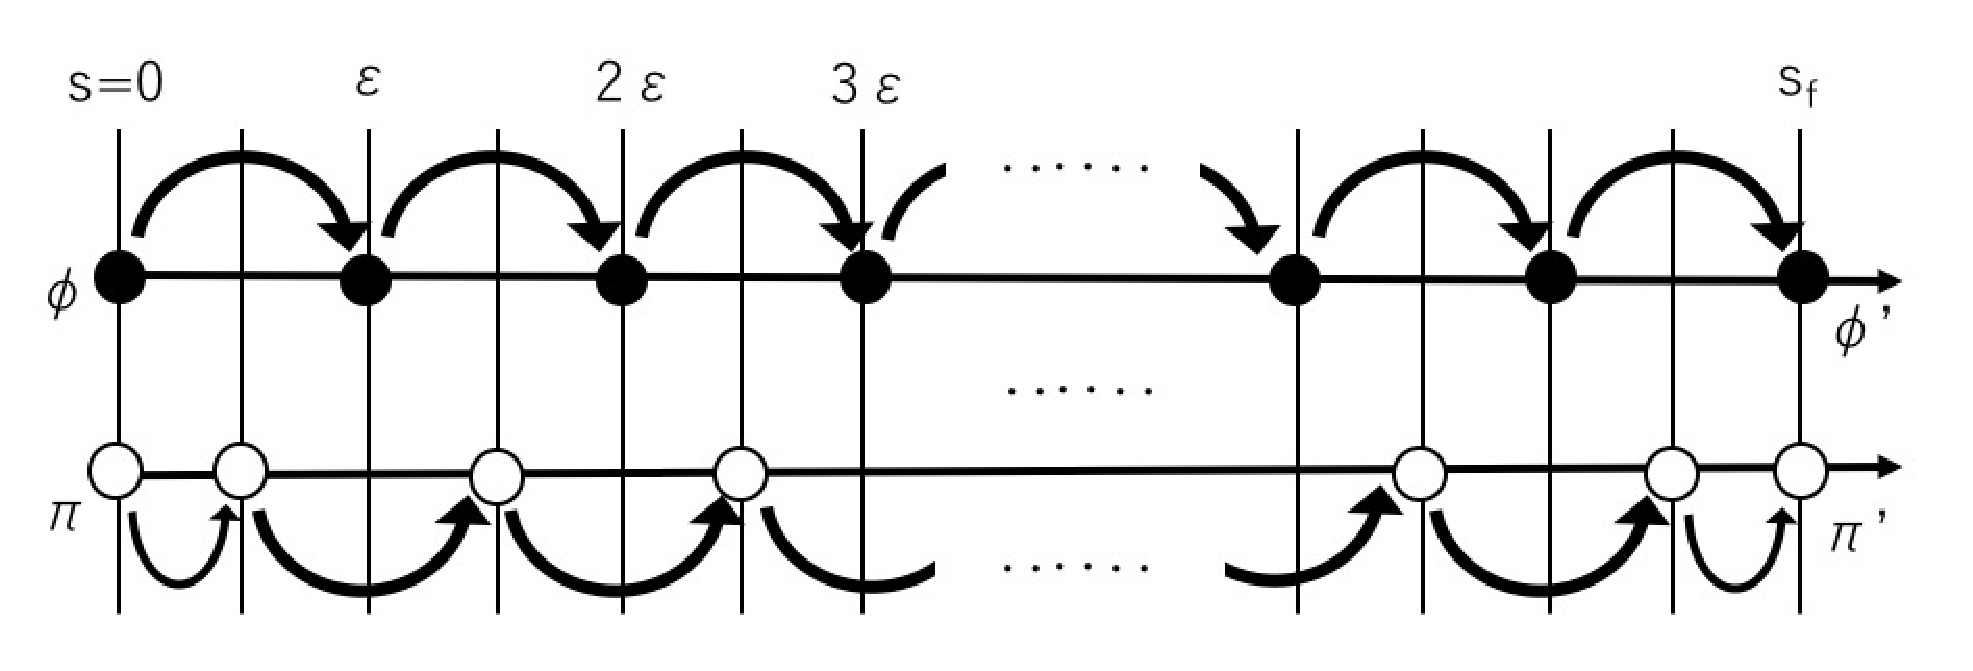
\includegraphics[scale=0.3]{Chapter3-figures/leapfrog.eps} 
 \end{center}
\caption{The leapfrog integrator.}
\label{fig:LF}
\end{figure}


%%%% references %%%%%%%%%
\begin{thebibliography}{99.}%

\bibitem{Wilson:1974sk}
  K.~G.~Wilson,
 ``Confinement of Quarks,''
  Phys.\ Rev.\ D {\bf 10} (1974) 2445.
  
 \bibitem{Creutz:1980zw}
  M.~Creutz,
  ``Monte Carlo Study of Quantized SU(2) Gauge Theory,''
  Phys.\ Rev.\ D {\bf 21} (1980) 2308. 
  
  \bibitem{Brambilla:2014jmp}
  N.~Brambilla {\it et al.},
  ``QCD and Strongly Coupled Gauge Theories: Challenges and Perspectives,''
  Eur.\ Phys.\ J.\ C {\bf 74} (2014) 2981
 %doi:10.1140/epjc/s10052-014-2981-5
  [arXiv:1404.3723 [hep-ph]].
   
  \bibitem{Wilson:2004de}
  K.~G.~Wilson,
  ``The Origins of lattice gauge theory,''
  Nucl.\ Phys.\ Proc.\ Suppl.\  {\bf 140} (2005) 3
  %doi:10.1016/j.nuclphysbps.2004.11.271
  [hep-lat/0412043].
  
\bibitem{Creutz:1984mg}
  M.~Creutz,
  ``Quarks, gluons and lattices,''
  Cambridge Monographs on Mathematical Physics (Cambridge Univ. Press, UK, 1985) pp. 1-169.
    
\bibitem{Rothe:1992nt}
  H.~J.~Rothe,
  ``Lattice gauge theories: An Introduction,''
 World Sci.\ Lect.\ Notes Phys. vol.82 (2012) pp. 1-606.
  %%CITATION = 00327,43,1;%%  

 \bibitem{Hoelbling:2014uea}
  C.~Hoelbling,
  ``Lattice QCD: concepts, techniques and some results,''
  Acta Phys.\ Polon.\ B {\bf 45} (2014)  2143
 % doi:10.5506/APhysPolB.45.2143
  [arXiv:1410.3403 [hep-lat]]. 

 \bibitem{Ukawa:2015eka}
  A.~Ukawa,
  ``Kenneth Wilson and lattice QCD,''
  J.\ Statist.\ Phys.\  {\bf 160} (2015) 1081
 % doi:10.1007/s10955-015-1197-x
  [arXiv:1501.04215 [hep-lat]]. 
 
\bibitem{Negele:1988vy}
  J.~W.~Negele and H.~Orland,
  ``Quantum Many Particle Systems,''
  FRONTIERS IN PHYSICS, vol.68 (Addison-Wesley, USA, 1988) pp. 1-459.    

\bibitem{Haggstrom:2002}
  O. H\"{a}ggstr\"{o}m,
  ``Finite Markov Chains and Algorithmic Applications,''
 London Mathematical Society, Student Texts, vol. 52   (Cambridge Univ. Press, UK, 2002) pp. 1-114.    

\bibitem{SuwaTodo:2010}
 H. Suwa and S.Todo,
 ``Markov Chain Monte Carlo Method without Detailed Balance,"
 Phys.\ Rev.\ Lett.\ {\bf 105} (2010) 120603
 [ArXiv:1007.2262 [cond-mat]].

 \bibitem{Duane:1987de}
  S.~Duane, A.~D.~Kennedy, B.~J.~Pendleton and D.~Roweth,
  ``Hybrid Monte Carlo,''
  Phys.\ Lett.\ B {\bf 195} (1987) 216.
%  doi:10.1016/0370-2693(87)91197-X
  
\bibitem{Metropolis_1953}
 N. Metropolis, A. W. Rosenbluth, M. N. Rosenbluth, A. H. Teller and E. Teller,
 ``Equation of State Calculations by Fast Computing Machines,''
 J. Chem. Phys. {\bf 21} (1953) 1087.
 %http://dx.doi.org/10.1063/1.1699114 
  
\bibitem{Schaefer:2012tq}
  S.~Schaefer,
 ``Status and challenges of simulations with dynamical fermions,''
  PoS LATTICE {\bf 2012} (2012) 001
  [arXiv:1211.5069 [hep-lat]].  
  
 \bibitem{Bali:2000gf}
  G.~S.~Bali,
  ``QCD forces and heavy quark bound states,''
  Phys.\ Rept.\  {\bf 343} (2001) 1
%  doi:10.1016/S0370-1573(00)00079-X
  [hep-ph/0001312]. 

\bibitem{Durr:2008zz}
  S.~Durr {\it et al.},
  ``Ab-Initio Determination of Light Hadron Masses,''
  Science {\bf 322} (2008) 1224
 % doi:10.1126/science.1163233
  [arXiv:0906.3599 [hep-lat]].
  
\bibitem{Borsanyi:2014jba}
  S.~Borsanyi {\it et al.},
 ``Ab initio calculation of the neutron-proton mass difference,''
  Science {\bf 347} (2015) 1452
%  doi:10.1126/science.1257050
  [arXiv:1406.4088 [hep-lat]].  
  
\bibitem{RPP}   
The Review of Particle Physics (2015),
\url{http://pdg.lbl.gov/ } 
  
\bibitem{Asakawa:2000tr}
  M.~Asakawa, T.~Hatsuda and Y.~Nakahara,
 ``Maximum entropy analysis of the spectral functions in lattice QCD,''
  Prog.\ Part.\ Nucl.\ Phys.\  {\bf 46} (2001) 459
 % doi:10.1016/S0146-6410(01)00150-8
  [hep-lat/0011040].
  
\bibitem{Fodor:2012gf}
  Z.~Fodor and C.~Hoelbling,
 ``Light Hadron Masses from Lattice QCD,''
  Rev.\ Mod.\ Phys.\  {\bf 84} (2012) 449
%  doi:10.1103/RevModPhys.84.449
  [arXiv:1203.4789 [hep-lat]].
   
\bibitem{this_book}
Consult other chapters of this volume.
 
 \bibitem{Machleidt:2007ms}
  R.~Machleidt,
  ``Nuclear forces from chiral effective field theory,''
  arXiv:0704.0807 [nucl-th].

\bibitem{Aoki:2013ldr}
  S.~Aoki {\it et al.},
  ``Review of lattice results concerning low-energy particle physics,''
  Eur.\ Phys.\ J.\ C {\bf 74} (2014) 2890
%  doi:10.1140/epjc/s10052-014-2890-7
  [arXiv:1310.8555 [hep-lat]].

\bibitem{luescher}
 M.~L\"{u}scher,
``Two particle states on a torus and their relation to the scattering matrix,''
Nucl. \ Phys.\ B {\bf 354} (1991) 531

\bibitem{Ishii:2006ec}
N.~Ishii, S.~Aoki and T.~Hatsuda,
``The Nuclear Force from Lattice QCD,''
Phys.\ Rev.\ Lett.\  {\bf 99} (2007) 022001

\bibitem{HALQCD:2012aa}
  N.~Ishii {\it et al.} [HAL QCD Collaboration],
"Hadron-hadron interactions from imaginary-time Nambu-Bethe-Salpeter wave function on the lattice,"
 Phys.\ Lett.\ B {\bf 712} (2012) 437
%\UTF{00A0}\UTF{00A0}doi:10.1016/j.physletb.2012.04.076
[arXiv:1203.3642 [hep-lat]].

\bibitem{Iritani:2015dhu}
T.~Iritani [HALQCD Collaboration],
``Lattice QCD studies on baryon interactions from L\"uscher's finite volume method and HAL QCD method,''
arXiv:1511.05246 [hep-lat].

\bibitem{okubo}
S. Okubo S, R.E. Marshak,
``Velocity dependence of the two-nucleon interaction,"
Ann. of Phys. {\bf 4} (1958) 166.

\bibitem{Oka-Fujiwara}
M. Oka, K. Shimizu, K. Yazaki, 
 ``Quark cluster model of baryon baryon interaction,''
 {\it Prog.\ Theor.\ Phys.\ Suppl.}\  {\bf 137}  (2000) 1.  
% Y. Fujiwara, Y. Suzuki and C. Nakamoto,
%  ``Baryon baryon interactions in the SU(6) quark model and their applications
%  to light nuclear systems,''
%  {\it Prog.\ Part.\ Nucl.\ Phys.}\  {\bf 58} (2007) 439.

\bibitem{Inoue:2011ai}
  T.~Inoue {\it et al.} [HAL QCD Collaboration],
  ``Two-Baryon Potentials and H-Dibaryon from 3-flavor Lattice QCD Simulations,''
  Nucl.\ Phys.\ A {\bf 881} (2012) 28
%  doi:10.1016/j.nuclphysa.2012.02.008
  [arXiv:1112.5926 [hep-lat]].
  
  \bibitem{Inoue:2013nfe}
  T.~Inoue {\it et al.} [HAL QCD Collaboration],
  ``Equation of State for Nucleonic Matter and its Quark Mass Dependence from the Nuclear Force in Lattice QCD,''
  Phys.\ Rev.\ Lett.\  {\bf 111} (2013)  112503
%  doi:10.1103/PhysRevLett.111.112503
  [arXiv:1307.0299 [hep-lat]].
  
 \bibitem{Akmal:1998cf}
  A.~Akmal, V.~R.~Pandharipande and D.~G.~Ravenhall,
  ``The Equation of state of nucleon matter and neutron star structure,''
  Phys.\ Rev.\ C {\bf 58} (1998) 1804
%  doi:10.1103/PhysRevC.58.1804
  [nucl-th/9804027]. 
  
  \bibitem{Doi:2015oha}
  T.~Doi {\it et al.} [HAL QCD Collaboration],
  ``First results of baryon interactions from lattice QCD with physical masses (1) -- General overview and two-nucleon forces --,''
  arXiv:1512.01610 [hep-lat].
 


  
\end{thebibliography}
